\documentclass[twoside]{book}

% Packages required by doxygen
\usepackage{fixltx2e}
\usepackage{calc}
\usepackage{doxygen}
\usepackage[export]{adjustbox} % also loads graphicx
\usepackage{graphicx}
\usepackage[utf8]{inputenc}
\usepackage{makeidx}
\usepackage{multicol}
\usepackage{multirow}
\PassOptionsToPackage{warn}{textcomp}
\usepackage{textcomp}
\usepackage[nointegrals]{wasysym}
\usepackage[table]{xcolor}

% Font selection
\usepackage[T1]{fontenc}
\usepackage[scaled=.90]{helvet}
\usepackage{courier}
\usepackage{amssymb}
\usepackage{sectsty}
\renewcommand{\familydefault}{\sfdefault}
\allsectionsfont{%
  \fontseries{bc}\selectfont%
  \color{darkgray}%
}
\renewcommand{\DoxyLabelFont}{%
  \fontseries{bc}\selectfont%
  \color{darkgray}%
}
\newcommand{\+}{\discretionary{\mbox{\scriptsize$\hookleftarrow$}}{}{}}

% Page & text layout
\usepackage{geometry}
\geometry{%
  a4paper,%
  top=2.5cm,%
  bottom=2.5cm,%
  left=2.5cm,%
  right=2.5cm%
}
\tolerance=750
\hfuzz=15pt
\hbadness=750
\setlength{\emergencystretch}{15pt}
\setlength{\parindent}{0cm}
\setlength{\parskip}{3ex plus 2ex minus 2ex}
\makeatletter
\renewcommand{\paragraph}{%
  \@startsection{paragraph}{4}{0ex}{-1.0ex}{1.0ex}{%
    \normalfont\normalsize\bfseries\SS@parafont%
  }%
}
\renewcommand{\subparagraph}{%
  \@startsection{subparagraph}{5}{0ex}{-1.0ex}{1.0ex}{%
    \normalfont\normalsize\bfseries\SS@subparafont%
  }%
}
\makeatother

% Headers & footers
\usepackage{fancyhdr}
\pagestyle{fancyplain}
\fancyhead[LE]{\fancyplain{}{\bfseries\thepage}}
\fancyhead[CE]{\fancyplain{}{}}
\fancyhead[RE]{\fancyplain{}{\bfseries\leftmark}}
\fancyhead[LO]{\fancyplain{}{\bfseries\rightmark}}
\fancyhead[CO]{\fancyplain{}{}}
\fancyhead[RO]{\fancyplain{}{\bfseries\thepage}}
\fancyfoot[LE]{\fancyplain{}{}}
\fancyfoot[CE]{\fancyplain{}{}}
\fancyfoot[RE]{\fancyplain{}{\bfseries\scriptsize Generated by Doxygen }}
\fancyfoot[LO]{\fancyplain{}{\bfseries\scriptsize Generated by Doxygen }}
\fancyfoot[CO]{\fancyplain{}{}}
\fancyfoot[RO]{\fancyplain{}{}}
\renewcommand{\footrulewidth}{0.4pt}
\renewcommand{\chaptermark}[1]{%
  \markboth{#1}{}%
}
\renewcommand{\sectionmark}[1]{%
  \markright{\thesection\ #1}%
}

% Indices & bibliography
\usepackage{natbib}
\usepackage[titles]{tocloft}
\setcounter{tocdepth}{3}
\setcounter{secnumdepth}{5}
\makeindex

% Hyperlinks (required, but should be loaded last)
\usepackage{ifpdf}
\ifpdf
  \usepackage[pdftex,pagebackref=true]{hyperref}
\else
  \usepackage[ps2pdf,pagebackref=true]{hyperref}
\fi
\hypersetup{%
  colorlinks=true,%
  linkcolor=blue,%
  citecolor=blue,%
  unicode%
}

% Custom commands
\newcommand{\clearemptydoublepage}{%
  \newpage{\pagestyle{empty}\cleardoublepage}%
}

\usepackage{caption}
\captionsetup{labelsep=space,justification=centering,font={bf},singlelinecheck=off,skip=4pt,position=top}

%===== C O N T E N T S =====

\begin{document}

% Titlepage & ToC
\hypersetup{pageanchor=false,
             bookmarksnumbered=true,
             pdfencoding=unicode
            }
\pagenumbering{alph}
\begin{titlepage}
\vspace*{7cm}
\begin{center}%
{\Large S\+I\+TS \\[1ex]\large .101 }\\
\vspace*{1cm}
{\large Generated by Doxygen 1.8.13}\\
\end{center}
\end{titlepage}
\clearemptydoublepage
\pagenumbering{roman}
\tableofcontents
\clearemptydoublepage
\pagenumbering{arabic}
\hypersetup{pageanchor=true}

%--- Begin generated contents ---
\chapter{S\+I\+TS}
\label{md__r_e_a_d_m_e}
\Hypertarget{md__r_e_a_d_m_e}
Synthetic Aperture Radar Image Testing Suite 
\chapter{Hierarchical Index}
\section{Class Hierarchy}
This inheritance list is sorted roughly, but not completely, alphabetically\+:\begin{DoxyCompactList}
\item \contentsline{section}{Antenna}{\pageref{class_antenna}}{}
\item \contentsline{section}{Data\+Generator}{\pageref{class_data_generator}}{}
\begin{DoxyCompactList}
\item \contentsline{section}{Data\+Generator2d}{\pageref{class_data_generator2d}}{}
\end{DoxyCompactList}
\item \contentsline{section}{Image\+Recoverer}{\pageref{class_image_recoverer}}{}
\begin{DoxyCompactList}
\item \contentsline{section}{Image\+Recoverer2d}{\pageref{class_image_recoverer2d}}{}
\item \contentsline{section}{Image\+Recoverer3d}{\pageref{class_image_recoverer3d}}{}
\item \contentsline{section}{Image\+Recoverer\+Direct}{\pageref{class_image_recoverer_direct}}{}
\end{DoxyCompactList}
\item \contentsline{section}{Imaging\+Plane}{\pageref{class_imaging_plane}}{}
\item \contentsline{section}{Math}{\pageref{class_math}}{}
\item \contentsline{section}{S\+AR}{\pageref{class_s_a_r}}{}
\item \contentsline{section}{Signal}{\pageref{class_signal}}{}
\begin{DoxyCompactList}
\item \contentsline{section}{Chirp}{\pageref{class_chirp}}{}
\item \contentsline{section}{Rect}{\pageref{class_rect}}{}
\end{DoxyCompactList}
\item \contentsline{section}{Target}{\pageref{class_target}}{}
\begin{DoxyCompactList}
\item \contentsline{section}{Target2dF}{\pageref{class_target2d_f}}{}
\item \contentsline{section}{Target2dS}{\pageref{class_target2d_s}}{}
\item \contentsline{section}{Target3dS}{\pageref{class_target3d_s}}{}
\end{DoxyCompactList}
\end{DoxyCompactList}

\chapter{Class Index}
\section{Class List}
Here are the classes, structs, unions and interfaces with brief descriptions\+:\begin{DoxyCompactList}
\item\contentsline{section}{\hyperlink{class_antenna}{Antenna} }{\pageref{class_antenna}}{}
\item\contentsline{section}{\hyperlink{class_chirp}{Chirp} }{\pageref{class_chirp}}{}
\item\contentsline{section}{\hyperlink{class_data_generator}{Data\+Generator} }{\pageref{class_data_generator}}{}
\item\contentsline{section}{\hyperlink{class_data_generator2d}{Data\+Generator2d} }{\pageref{class_data_generator2d}}{}
\item\contentsline{section}{\hyperlink{class_image_recoverer}{Image\+Recoverer} }{\pageref{class_image_recoverer}}{}
\item\contentsline{section}{\hyperlink{class_image_recoverer2d}{Image\+Recoverer2d} }{\pageref{class_image_recoverer2d}}{}
\item\contentsline{section}{\hyperlink{class_image_recoverer3d}{Image\+Recoverer3d} }{\pageref{class_image_recoverer3d}}{}
\item\contentsline{section}{\hyperlink{class_image_recoverer_direct}{Image\+Recoverer\+Direct} }{\pageref{class_image_recoverer_direct}}{}
\item\contentsline{section}{\hyperlink{class_imaging_plane}{Imaging\+Plane} \\*The plane that }{\pageref{class_imaging_plane}}{}
\item\contentsline{section}{\hyperlink{class_math}{Math} }{\pageref{class_math}}{}
\item\contentsline{section}{\hyperlink{class_rect}{Rect} }{\pageref{class_rect}}{}
\item\contentsline{section}{\hyperlink{class_s_a_r}{S\+AR} }{\pageref{class_s_a_r}}{}
\item\contentsline{section}{\hyperlink{class_signal}{Signal} \\*Represents the signal that the antenna will modulate and apply as a current to the }{\pageref{class_signal}}{}
\item\contentsline{section}{\hyperlink{class_target}{Target} }{\pageref{class_target}}{}
\item\contentsline{section}{\hyperlink{class_target2d_f}{Target2dF} }{\pageref{class_target2d_f}}{}
\item\contentsline{section}{\hyperlink{class_target2d_s}{Target2dS} }{\pageref{class_target2d_s}}{}
\item\contentsline{section}{\hyperlink{class_target3d_s}{Target3dS} }{\pageref{class_target3d_s}}{}
\end{DoxyCompactList}

\chapter{File Index}
\section{File List}
Here is a list of all files with brief descriptions\+:\begin{DoxyCompactList}
\item\contentsline{section}{Data\+\_\+\+Generator/\hyperlink{_data___generator_8cpp}{Data\+\_\+\+Generator.\+cpp} }{\pageref{_data___generator_8cpp}}{}
\item\contentsline{section}{Data\+\_\+\+Generator/\hyperlink{_data___generator_8h}{Data\+\_\+\+Generator.\+h} }{\pageref{_data___generator_8h}}{}
\item\contentsline{section}{Image\+\_\+\+Recovery/\hyperlink{_image___recoverer_8cpp}{Image\+\_\+\+Recoverer.\+cpp} }{\pageref{_image___recoverer_8cpp}}{}
\item\contentsline{section}{Image\+\_\+\+Recovery/\hyperlink{_image___recoverer_8h}{Image\+\_\+\+Recoverer.\+h} }{\pageref{_image___recoverer_8h}}{}
\item\contentsline{section}{Image\+\_\+\+Recovery/\hyperlink{_image___recoverer___butterfly_8h}{Image\+\_\+\+Recoverer\+\_\+\+Butterfly.\+h} }{\pageref{_image___recoverer___butterfly_8h}}{}
\item\contentsline{section}{Image\+\_\+\+Recovery/\hyperlink{_image___recoverer___direct_8h}{Image\+\_\+\+Recoverer\+\_\+\+Direct.\+h} }{\pageref{_image___recoverer___direct_8h}}{}
\item\contentsline{section}{lib/\hyperlink{_math_8h}{Math.\+h} }{\pageref{_math_8h}}{}
\item\contentsline{section}{lib/\hyperlink{_s_a_r_8h}{S\+A\+R.\+h} }{\pageref{_s_a_r_8h}}{}
\item\contentsline{section}{lib/\hyperlink{_target_8h}{Target.\+h} }{\pageref{_target_8h}}{}
\item\contentsline{section}{Target\+\_\+\+Generator/\hyperlink{_target_creator_8cpp}{Target\+Creator.\+cpp} }{\pageref{_target_creator_8cpp}}{}
\item\contentsline{section}{Target\+\_\+\+Generator/\hyperlink{_target_editor_8cpp}{Target\+Editor.\+cpp} }{\pageref{_target_editor_8cpp}}{}
\item\contentsline{section}{test/\hyperlink{test_8cpp}{test.\+cpp} }{\pageref{test_8cpp}}{}
\item\contentsline{section}{test/\hyperlink{test_8h}{test.\+h} }{\pageref{test_8h}}{}
\item\contentsline{section}{Testing/\hyperlink{_data___generation___unit___test_8cpp}{Data\+\_\+\+Generation\+\_\+\+Unit\+\_\+\+Test.\+cpp} }{\pageref{_data___generation___unit___test_8cpp}}{}
\item\contentsline{section}{Testing/\hyperlink{_image___editor___unit___test_8cpp}{Image\+\_\+\+Editor\+\_\+\+Unit\+\_\+\+Test.\+cpp} }{\pageref{_image___editor___unit___test_8cpp}}{}
\item\contentsline{section}{Testing/\hyperlink{_target___recovery___unit___test_8cpp}{Target\+\_\+\+Recovery\+\_\+\+Unit\+\_\+\+Test.\+cpp} }{\pageref{_target___recovery___unit___test_8cpp}}{}
\end{DoxyCompactList}

\chapter{Class Documentation}
\hypertarget{class_antenna}{}\section{Antenna Class Reference}
\label{class_antenna}\index{Antenna@{Antenna}}


{\ttfamily \#include $<$S\+A\+R.\+h$>$}



\subsection{Detailed Description}
\hyperlink{class_antenna}{Antenna} can act as tranmitter or reciever. As tranmitter, it takes the signal and creates an incident field. As reciever, it integrates the field incident on the antenna support. 

Definition at line 80 of file S\+A\+R.\+h.



The documentation for this class was generated from the following file\+:\begin{DoxyCompactItemize}
\item 
lib/\hyperlink{_s_a_r_8h}{S\+A\+R.\+h}\end{DoxyCompactItemize}

\hypertarget{class_chirp}{}\section{Chirp Class Reference}
\label{class_chirp}\index{Chirp@{Chirp}}


{\ttfamily \#include $<$S\+A\+R.\+h$>$}

Inheritance diagram for Chirp\+:\begin{figure}[H]
\begin{center}
\leavevmode
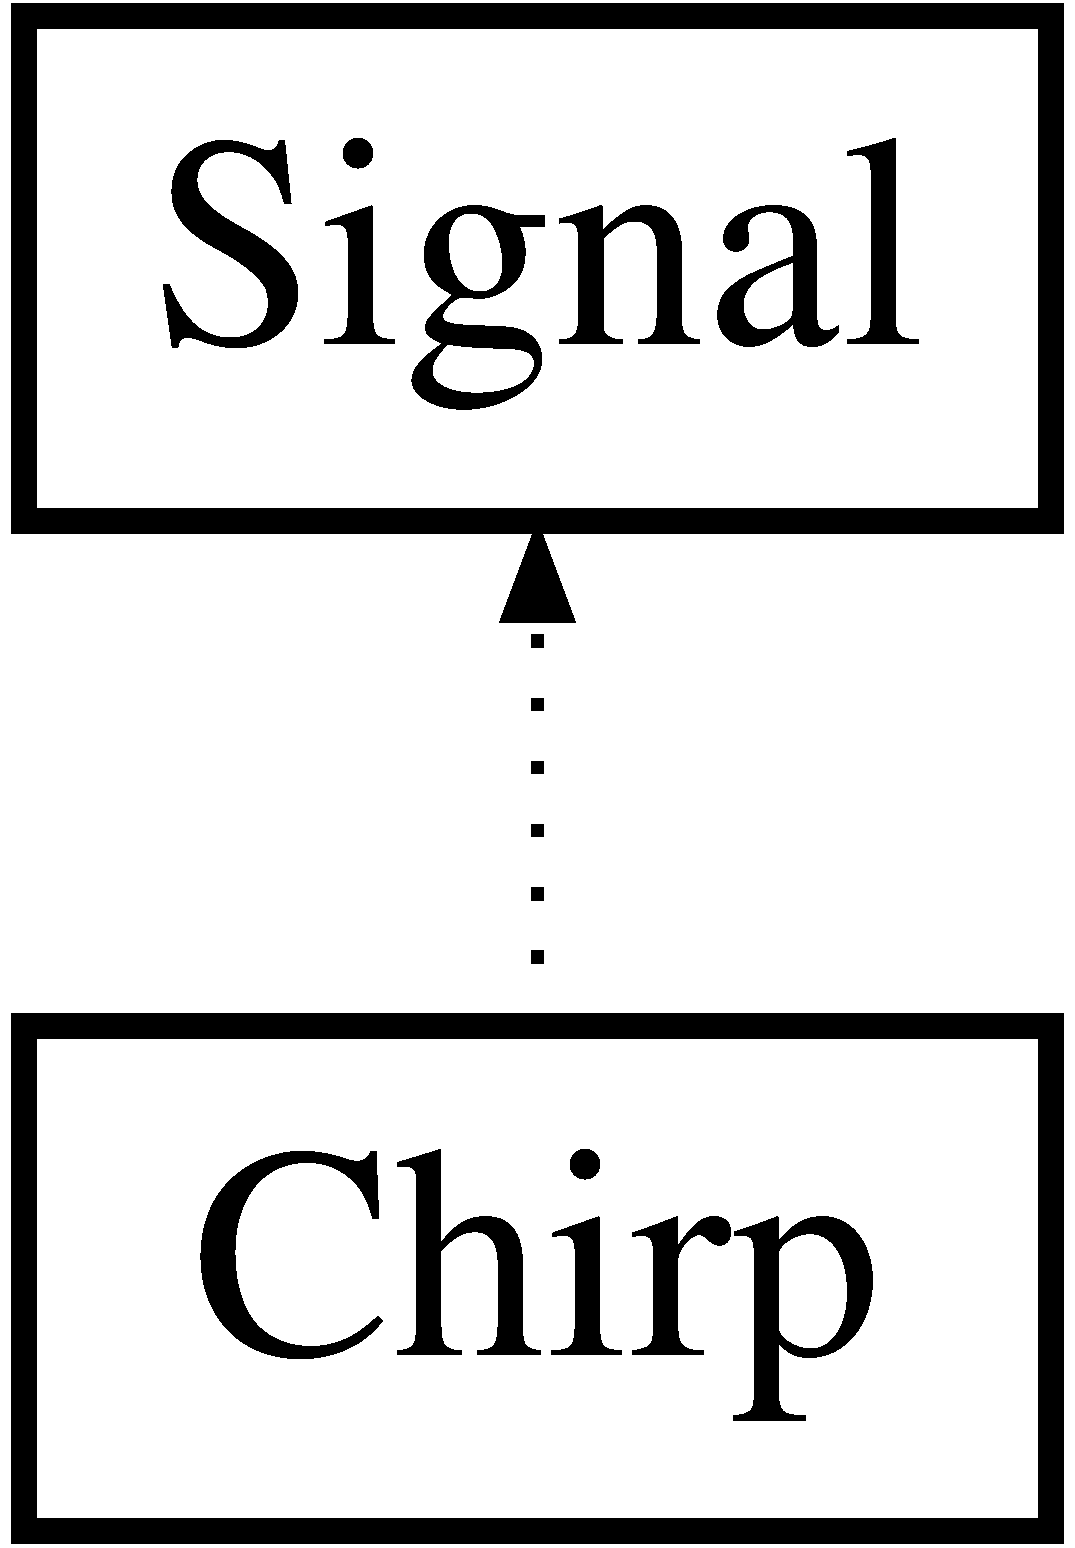
\includegraphics[height=2.000000cm]{class_chirp}
\end{center}
\end{figure}


\subsection{Detailed Description}


Definition at line 48 of file S\+A\+R.\+h.



The documentation for this class was generated from the following file\+:\begin{DoxyCompactItemize}
\item 
lib/\hyperlink{_s_a_r_8h}{S\+A\+R.\+h}\end{DoxyCompactItemize}

\hypertarget{class_data_generator}{}\section{Data\+Generator Class Reference}
\label{class_data_generator}\index{Data\+Generator@{Data\+Generator}}


{\ttfamily \#include $<$Data\+\_\+\+Generator.\+h$>$}

Inheritance diagram for Data\+Generator\+:\begin{figure}[H]
\begin{center}
\leavevmode
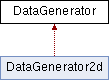
\includegraphics[height=2.000000cm]{class_data_generator}
\end{center}
\end{figure}


\subsection{Detailed Description}


Definition at line 22 of file Data\+\_\+\+Generator.\+h.



The documentation for this class was generated from the following file\+:\begin{DoxyCompactItemize}
\item 
Data\+\_\+\+Generator/\hyperlink{_data___generator_8h}{Data\+\_\+\+Generator.\+h}\end{DoxyCompactItemize}

\hypertarget{class_data_generator2d}{}\section{Data\+Generator2d Class Reference}
\label{class_data_generator2d}\index{Data\+Generator2d@{Data\+Generator2d}}


{\ttfamily \#include $<$Data\+\_\+\+Generator.\+h$>$}

Inheritance diagram for Data\+Generator2d\+:\begin{figure}[H]
\begin{center}
\leavevmode
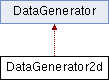
\includegraphics[height=2.000000cm]{class_data_generator2d}
\end{center}
\end{figure}


\subsection{Detailed Description}


Definition at line 37 of file Data\+\_\+\+Generator.\+h.



The documentation for this class was generated from the following file\+:\begin{DoxyCompactItemize}
\item 
Data\+\_\+\+Generator/\hyperlink{_data___generator_8h}{Data\+\_\+\+Generator.\+h}\end{DoxyCompactItemize}

\hypertarget{class_image_recoverer}{}\section{Image\+Recoverer Class Reference}
\label{class_image_recoverer}\index{Image\+Recoverer@{Image\+Recoverer}}


{\ttfamily \#include $<$Image\+\_\+\+Recoverer.\+h$>$}

Inheritance diagram for Image\+Recoverer\+:\begin{figure}[H]
\begin{center}
\leavevmode
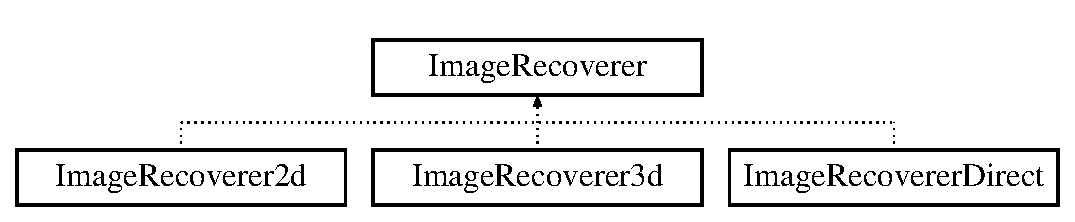
\includegraphics[height=2.000000cm]{class_image_recoverer}
\end{center}
\end{figure}


\subsection{Detailed Description}
Take a given sar system and convert its collected data into an estimate for the object that create that data. This is an abstract class. Actually recoverying and image depends on the geometry of the scenario and collected data. 

Definition at line 13 of file Image\+\_\+\+Recoverer.\+h.



The documentation for this class was generated from the following file\+:\begin{DoxyCompactItemize}
\item 
Image\+\_\+\+Recovery/\hyperlink{_image___recoverer_8h}{Image\+\_\+\+Recoverer.\+h}\end{DoxyCompactItemize}

\hypertarget{class_image_recoverer2d}{}\section{Image\+Recoverer2d Class Reference}
\label{class_image_recoverer2d}\index{Image\+Recoverer2d@{Image\+Recoverer2d}}


{\ttfamily \#include $<$Image\+\_\+\+Recoverer.\+h$>$}

Inheritance diagram for Image\+Recoverer2d\+:\begin{figure}[H]
\begin{center}
\leavevmode
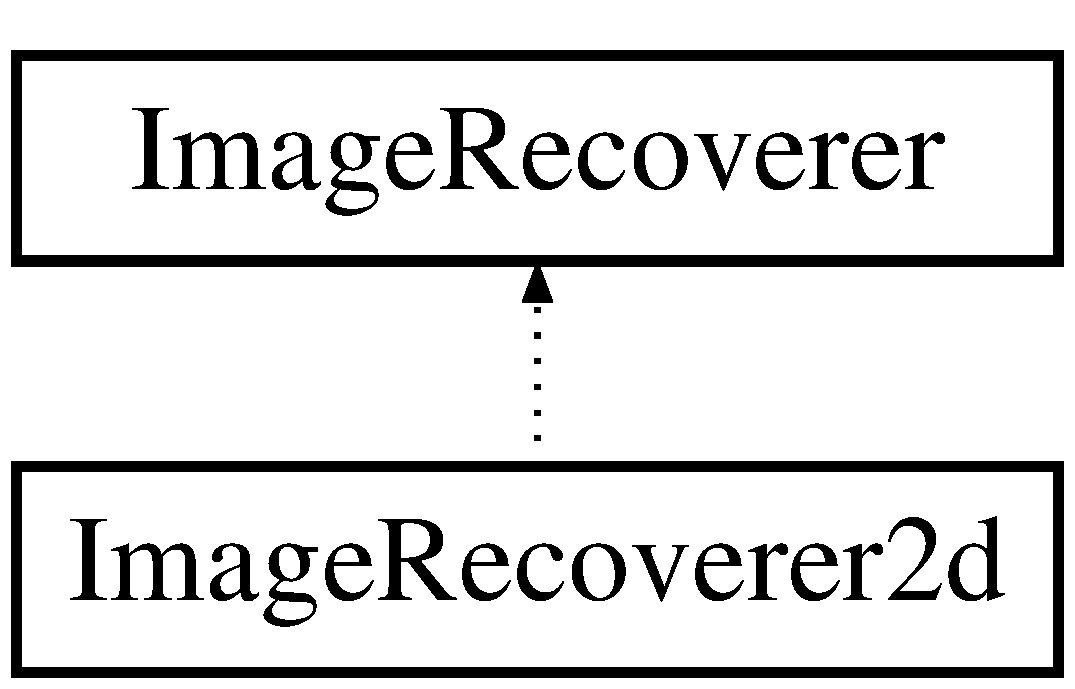
\includegraphics[height=2.000000cm]{class_image_recoverer2d}
\end{center}
\end{figure}


\subsection{Detailed Description}


Definition at line 33 of file Image\+\_\+\+Recoverer.\+h.



The documentation for this class was generated from the following file\+:\begin{DoxyCompactItemize}
\item 
Image\+\_\+\+Recovery/\hyperlink{_image___recoverer_8h}{Image\+\_\+\+Recoverer.\+h}\end{DoxyCompactItemize}

\hypertarget{class_image_recoverer3d}{}\section{Image\+Recoverer3d Class Reference}
\label{class_image_recoverer3d}\index{Image\+Recoverer3d@{Image\+Recoverer3d}}


{\ttfamily \#include $<$Image\+\_\+\+Recoverer.\+h$>$}

Inheritance diagram for Image\+Recoverer3d\+:\begin{figure}[H]
\begin{center}
\leavevmode
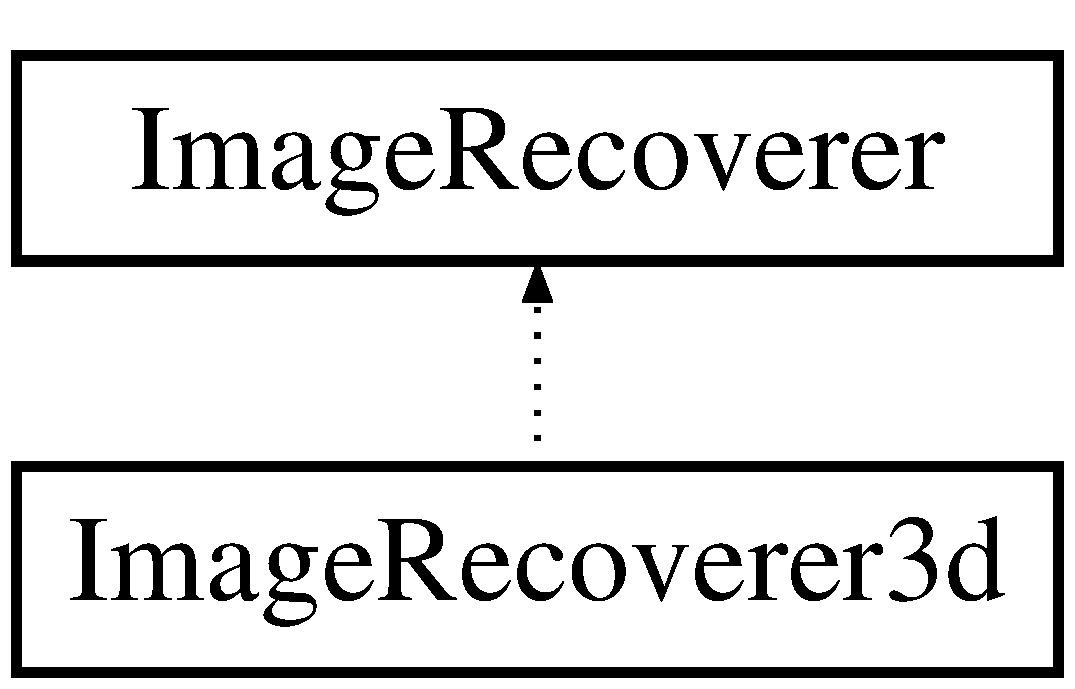
\includegraphics[height=2.000000cm]{class_image_recoverer3d}
\end{center}
\end{figure}


\subsection{Detailed Description}


Definition at line 35 of file Image\+\_\+\+Recoverer.\+h.



The documentation for this class was generated from the following file\+:\begin{DoxyCompactItemize}
\item 
Image\+\_\+\+Recovery/\hyperlink{_image___recoverer_8h}{Image\+\_\+\+Recoverer.\+h}\end{DoxyCompactItemize}

\hypertarget{class_image_recoverer_direct}{}\section{Image\+Recoverer\+Direct Class Reference}
\label{class_image_recoverer_direct}\index{Image\+Recoverer\+Direct@{Image\+Recoverer\+Direct}}


{\ttfamily \#include $<$Image\+\_\+\+Recoverer\+\_\+\+Direct.\+h$>$}

Inheritance diagram for Image\+Recoverer\+Direct\+:\begin{figure}[H]
\begin{center}
\leavevmode
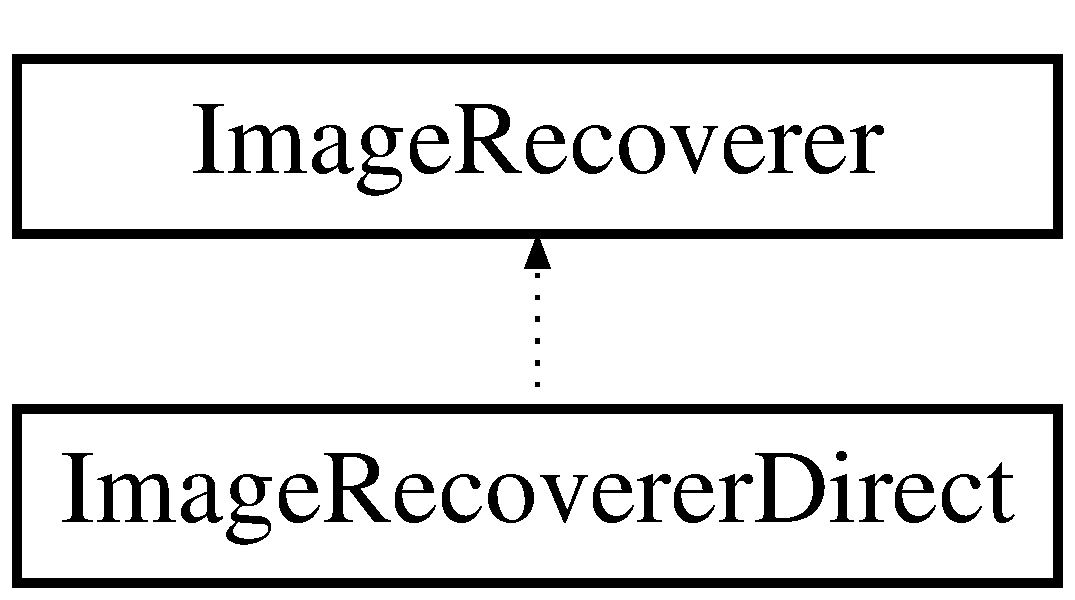
\includegraphics[height=2.000000cm]{class_image_recoverer_direct}
\end{center}
\end{figure}


\subsection{Detailed Description}


Definition at line 10 of file Image\+\_\+\+Recoverer\+\_\+\+Direct.\+h.



The documentation for this class was generated from the following file\+:\begin{DoxyCompactItemize}
\item 
Image\+\_\+\+Recovery/\hyperlink{_image___recoverer___direct_8h}{Image\+\_\+\+Recoverer\+\_\+\+Direct.\+h}\end{DoxyCompactItemize}

\hypertarget{class_imaging_plane}{}\section{Imaging\+Plane Class Reference}
\label{class_imaging_plane}\index{Imaging\+Plane@{Imaging\+Plane}}


The plane that.  




{\ttfamily \#include $<$Image\+\_\+\+Recoverer.\+h$>$}



\subsection{Detailed Description}
The plane that. 

Definition at line 29 of file Image\+\_\+\+Recoverer.\+h.



The documentation for this class was generated from the following file\+:\begin{DoxyCompactItemize}
\item 
Image\+\_\+\+Recovery/\hyperlink{_image___recoverer_8h}{Image\+\_\+\+Recoverer.\+h}\end{DoxyCompactItemize}

\hypertarget{class_math}{}\section{Math Class Reference}
\label{class_math}\index{Math@{Math}}


{\ttfamily \#include $<$Math.\+h$>$}



\subsection{Detailed Description}


Definition at line 5 of file Math.\+h.



The documentation for this class was generated from the following file\+:\begin{DoxyCompactItemize}
\item 
lib/\hyperlink{_math_8h}{Math.\+h}\end{DoxyCompactItemize}

\hypertarget{class_rect}{}\section{Rect Class Reference}
\label{class_rect}\index{Rect@{Rect}}


{\ttfamily \#include $<$S\+A\+R.\+h$>$}

Inheritance diagram for Rect\+:\begin{figure}[H]
\begin{center}
\leavevmode
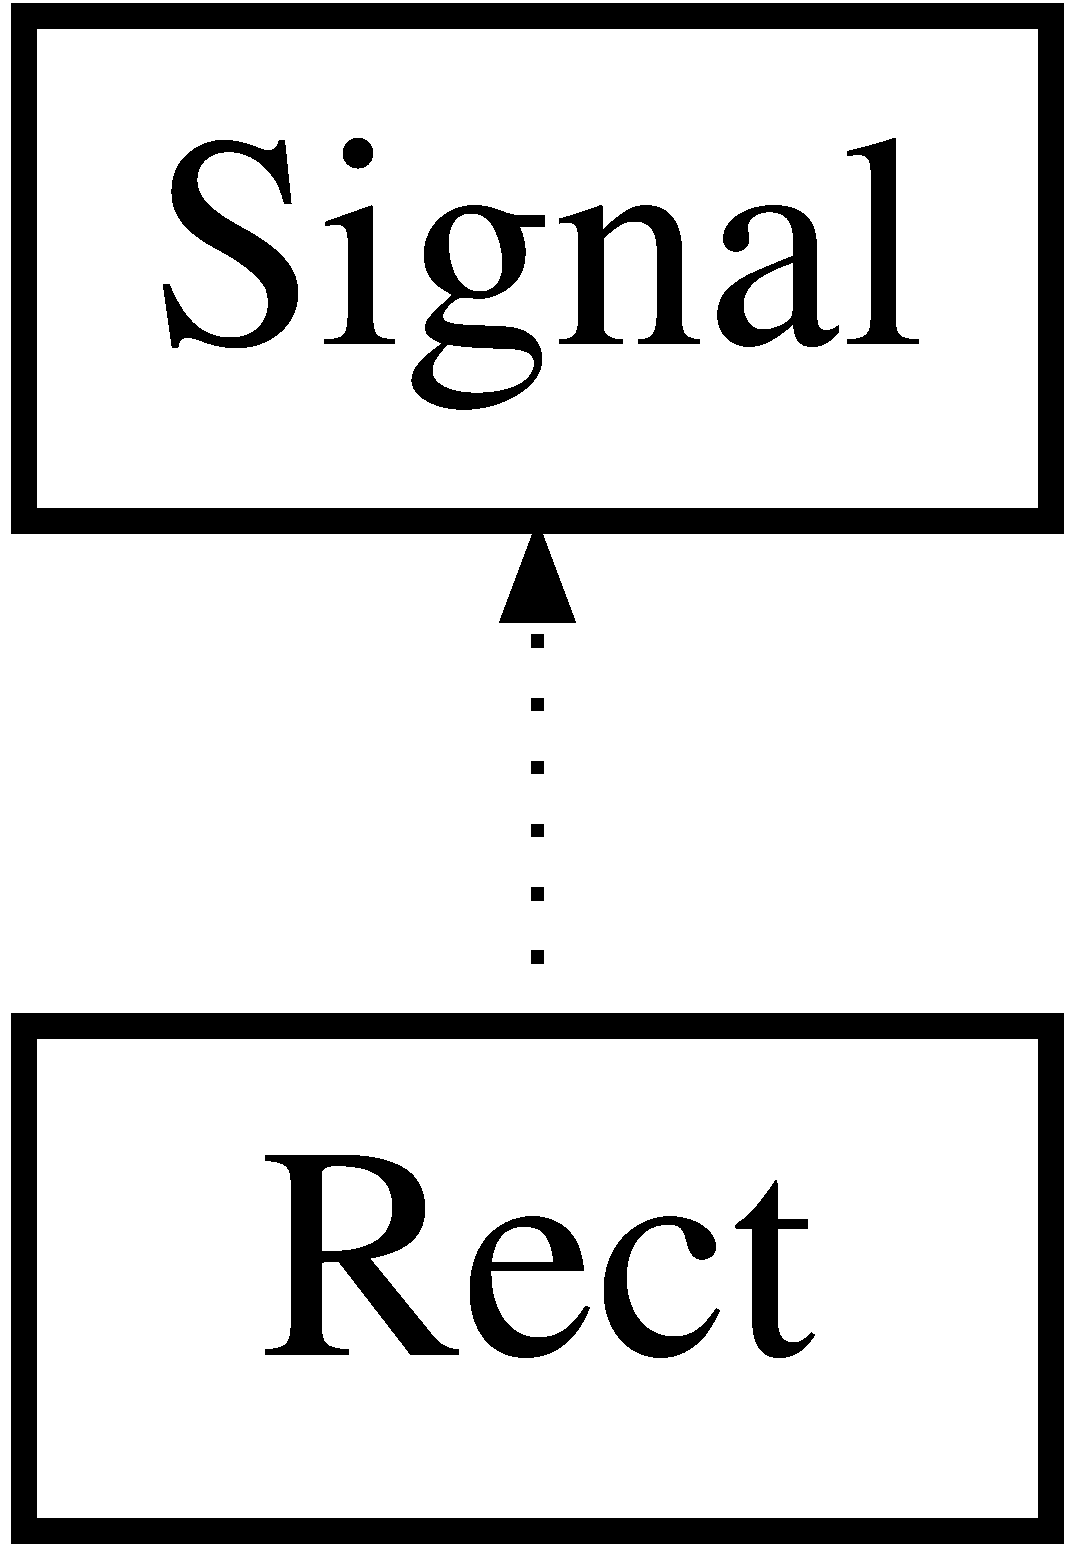
\includegraphics[height=2.000000cm]{class_rect}
\end{center}
\end{figure}


\subsection{Detailed Description}


Definition at line 65 of file S\+A\+R.\+h.



The documentation for this class was generated from the following file\+:\begin{DoxyCompactItemize}
\item 
lib/\hyperlink{_s_a_r_8h}{S\+A\+R.\+h}\end{DoxyCompactItemize}

\hypertarget{class_s_a_r}{}\section{S\+AR Class Reference}
\label{class_s_a_r}\index{S\+AR@{S\+AR}}


{\ttfamily \#include $<$S\+A\+R.\+h$>$}

\subsection*{Public Member Functions}
\begin{DoxyCompactItemize}
\item 
virtual point \hyperlink{class_s_a_r_ad8d31777e5b21cbfb75e5023830eb011}{flight\+\_\+path} (double t)
\end{DoxyCompactItemize}
\subsection*{Public Attributes}
\begin{DoxyCompactItemize}
\item 
\hyperlink{class_antenna}{Antenna} \hyperlink{class_s_a_r_a834de6d160196af5d7ea31c4140fb684}{antenna}
\item 
\hyperlink{class_signal}{Signal} \hyperlink{class_s_a_r_aa854bd6cbba87d014da962bea7a5e6d8}{p}
\item 
Carrier \hyperlink{class_s_a_r_a6108faaee083fa177cf3b837486a667f}{w0}
\item 
float \hyperlink{class_s_a_r_ad85918c46f8ea542f28a65a2f45b3962}{pulse\+\_\+rate}
\item 
float \hyperlink{class_s_a_r_aca187a89a350101ca7d1fad4d432f27b}{sample\+\_\+rate}
\item 
Data \hyperlink{class_s_a_r_a36a5fb0ba45e7fafc60cce11664fd81d}{data}
\end{DoxyCompactItemize}


\subsection{Detailed Description}


Definition at line 16 of file S\+A\+R.\+h.



\subsection{Member Function Documentation}
\mbox{\Hypertarget{class_s_a_r_ad8d31777e5b21cbfb75e5023830eb011}\label{class_s_a_r_ad8d31777e5b21cbfb75e5023830eb011}} 
\index{S\+AR@{S\+AR}!flight\+\_\+path@{flight\+\_\+path}}
\index{flight\+\_\+path@{flight\+\_\+path}!S\+AR@{S\+AR}}
\subsubsection{\texorpdfstring{flight\+\_\+path()}{flight\_path()}}
{\footnotesize\ttfamily virtual point S\+A\+R\+::flight\+\_\+path (\begin{DoxyParamCaption}\item[{double}]{t }\end{DoxyParamCaption})\hspace{0.3cm}{\ttfamily [virtual]}}



\subsection{Member Data Documentation}
\mbox{\Hypertarget{class_s_a_r_a834de6d160196af5d7ea31c4140fb684}\label{class_s_a_r_a834de6d160196af5d7ea31c4140fb684}} 
\index{S\+AR@{S\+AR}!antenna@{antenna}}
\index{antenna@{antenna}!S\+AR@{S\+AR}}
\subsubsection{\texorpdfstring{antenna}{antenna}}
{\footnotesize\ttfamily \hyperlink{class_antenna}{Antenna} S\+A\+R\+::antenna}



Definition at line 18 of file S\+A\+R.\+h.

\mbox{\Hypertarget{class_s_a_r_a36a5fb0ba45e7fafc60cce11664fd81d}\label{class_s_a_r_a36a5fb0ba45e7fafc60cce11664fd81d}} 
\index{S\+AR@{S\+AR}!data@{data}}
\index{data@{data}!S\+AR@{S\+AR}}
\subsubsection{\texorpdfstring{data}{data}}
{\footnotesize\ttfamily Data S\+A\+R\+::data}



Definition at line 25 of file S\+A\+R.\+h.

\mbox{\Hypertarget{class_s_a_r_aa854bd6cbba87d014da962bea7a5e6d8}\label{class_s_a_r_aa854bd6cbba87d014da962bea7a5e6d8}} 
\index{S\+AR@{S\+AR}!p@{p}}
\index{p@{p}!S\+AR@{S\+AR}}
\subsubsection{\texorpdfstring{p}{p}}
{\footnotesize\ttfamily \hyperlink{class_signal}{Signal} S\+A\+R\+::p}



Definition at line 20 of file S\+A\+R.\+h.

\mbox{\Hypertarget{class_s_a_r_ad85918c46f8ea542f28a65a2f45b3962}\label{class_s_a_r_ad85918c46f8ea542f28a65a2f45b3962}} 
\index{S\+AR@{S\+AR}!pulse\+\_\+rate@{pulse\+\_\+rate}}
\index{pulse\+\_\+rate@{pulse\+\_\+rate}!S\+AR@{S\+AR}}
\subsubsection{\texorpdfstring{pulse\+\_\+rate}{pulse\_rate}}
{\footnotesize\ttfamily float S\+A\+R\+::pulse\+\_\+rate}



Definition at line 22 of file S\+A\+R.\+h.

\mbox{\Hypertarget{class_s_a_r_aca187a89a350101ca7d1fad4d432f27b}\label{class_s_a_r_aca187a89a350101ca7d1fad4d432f27b}} 
\index{S\+AR@{S\+AR}!sample\+\_\+rate@{sample\+\_\+rate}}
\index{sample\+\_\+rate@{sample\+\_\+rate}!S\+AR@{S\+AR}}
\subsubsection{\texorpdfstring{sample\+\_\+rate}{sample\_rate}}
{\footnotesize\ttfamily float S\+A\+R\+::sample\+\_\+rate}



Definition at line 23 of file S\+A\+R.\+h.

\mbox{\Hypertarget{class_s_a_r_a6108faaee083fa177cf3b837486a667f}\label{class_s_a_r_a6108faaee083fa177cf3b837486a667f}} 
\index{S\+AR@{S\+AR}!w0@{w0}}
\index{w0@{w0}!S\+AR@{S\+AR}}
\subsubsection{\texorpdfstring{w0}{w0}}
{\footnotesize\ttfamily Carrier S\+A\+R\+::w0}



Definition at line 21 of file S\+A\+R.\+h.



The documentation for this class was generated from the following file\+:\begin{DoxyCompactItemize}
\item 
lib/\hyperlink{_s_a_r_8h}{S\+A\+R.\+h}\end{DoxyCompactItemize}

\hypertarget{class_signal}{}\section{Signal Class Reference}
\label{class_signal}\index{Signal@{Signal}}


Represents the signal that the antenna will modulate and apply as a current to the.  




{\ttfamily \#include $<$S\+A\+R.\+h$>$}

Inheritance diagram for Signal\+:\begin{figure}[H]
\begin{center}
\leavevmode
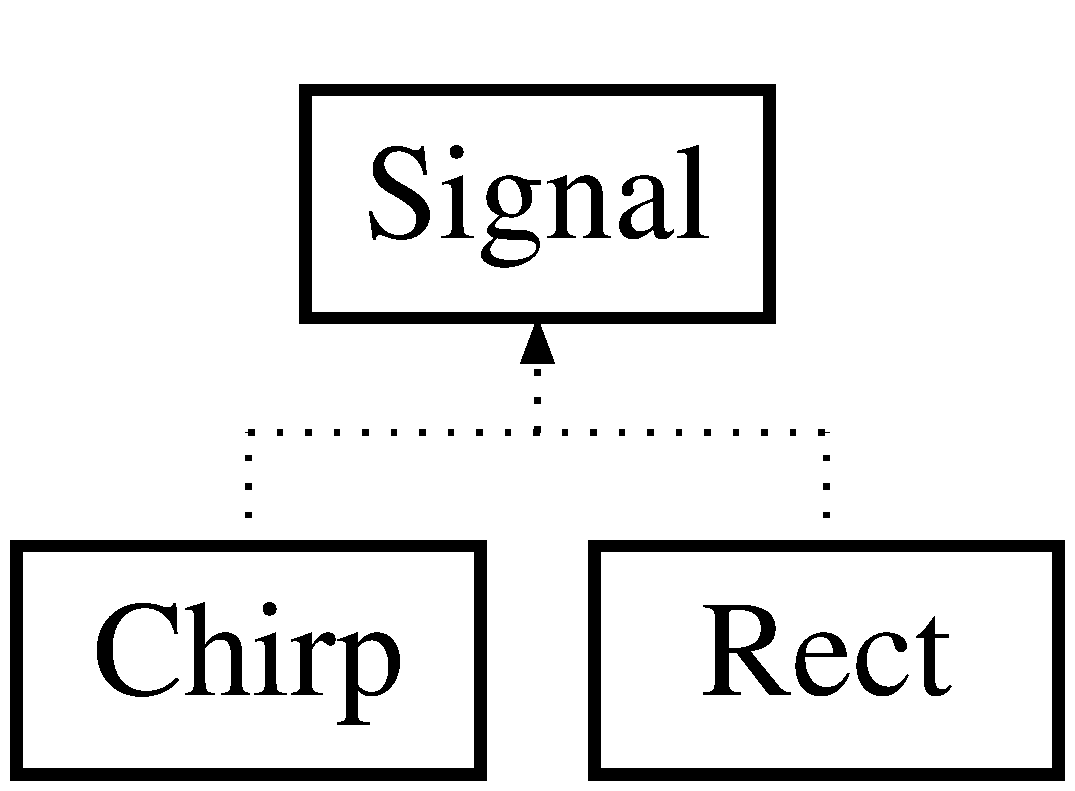
\includegraphics[height=2.000000cm]{class_signal}
\end{center}
\end{figure}


\subsection{Detailed Description}
Represents the signal that the antenna will modulate and apply as a current to the. 

Definition at line 33 of file S\+A\+R.\+h.



The documentation for this class was generated from the following file\+:\begin{DoxyCompactItemize}
\item 
lib/\hyperlink{_s_a_r_8h}{S\+A\+R.\+h}\end{DoxyCompactItemize}

\hypertarget{class_target}{}\section{Target Class Reference}
\label{class_target}\index{Target@{Target}}


{\ttfamily \#include $<$Target.\+h$>$}

Inheritance diagram for Target\+:\begin{figure}[H]
\begin{center}
\leavevmode
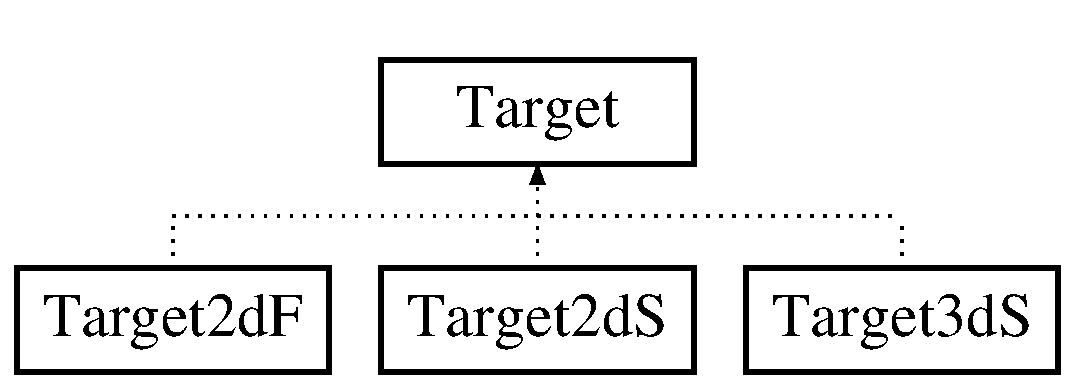
\includegraphics[height=2.000000cm]{class_target}
\end{center}
\end{figure}


\subsection{Detailed Description}
A target represents a physical entity that we would scatter an incident field. Currently, targets are assumed stationary. Subclasses include sampled targets, and function targets. A function target takes in a point and returns the reflectivity at that point. A sampled target is a discrete representation of the physical entity we are modeling. 

Definition at line 9 of file Target.\+h.



The documentation for this class was generated from the following file\+:\begin{DoxyCompactItemize}
\item 
lib/\hyperlink{_target_8h}{Target.\+h}\end{DoxyCompactItemize}

\hypertarget{class_target2d_f}{}\section{Target2dF Class Reference}
\label{class_target2d_f}\index{Target2dF@{Target2dF}}


{\ttfamily \#include $<$Target.\+h$>$}

Inheritance diagram for Target2dF\+:\begin{figure}[H]
\begin{center}
\leavevmode
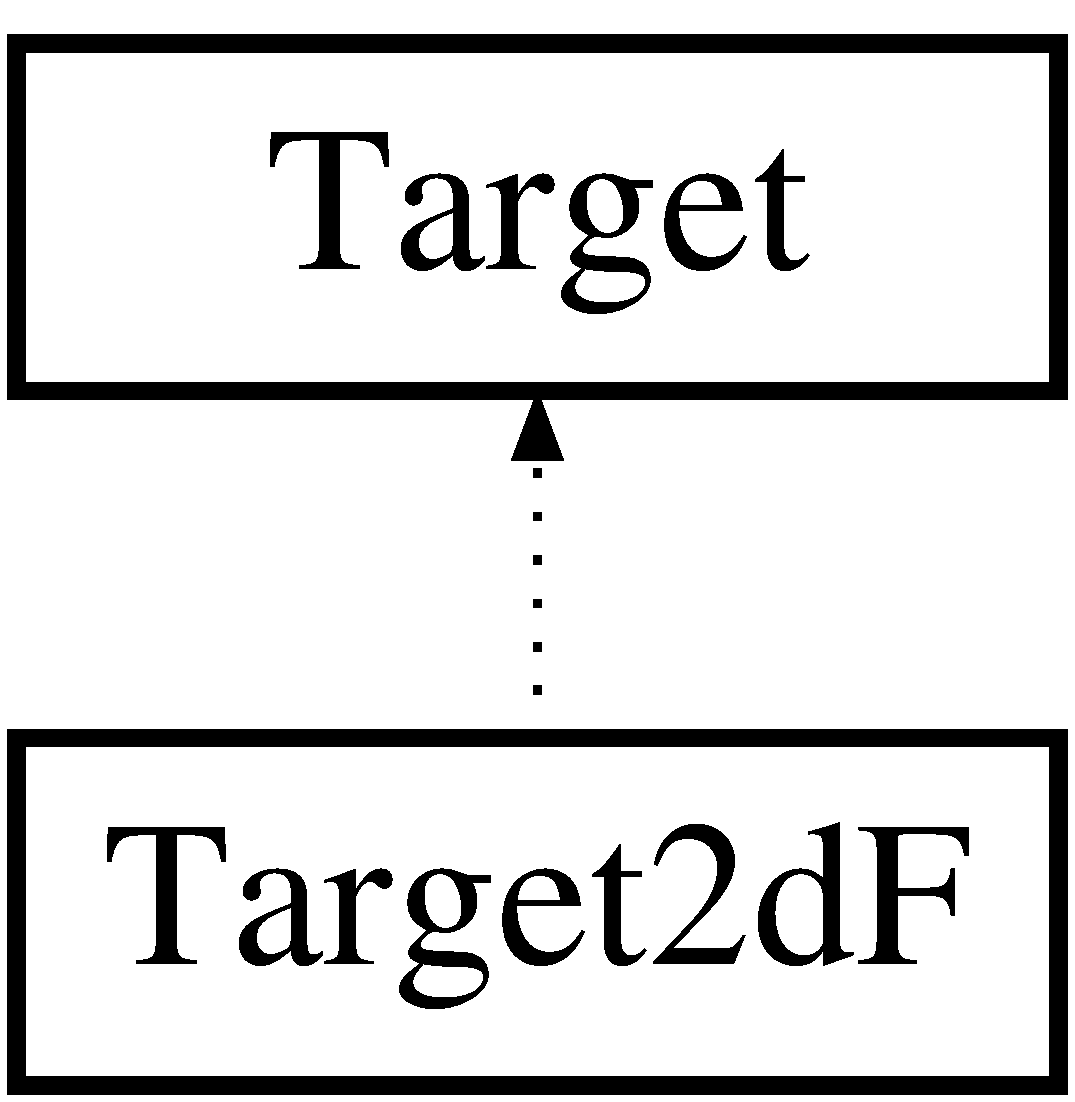
\includegraphics[height=2.000000cm]{class_target2d_f}
\end{center}
\end{figure}


\subsection{Detailed Description}


Definition at line 58 of file Target.\+h.



The documentation for this class was generated from the following file\+:\begin{DoxyCompactItemize}
\item 
lib/\hyperlink{_target_8h}{Target.\+h}\end{DoxyCompactItemize}

\hypertarget{class_target2d_s}{}\section{Target2dS Class Reference}
\label{class_target2d_s}\index{Target2dS@{Target2dS}}


{\ttfamily \#include $<$Target.\+h$>$}

Inheritance diagram for Target2dS\+:\begin{figure}[H]
\begin{center}
\leavevmode
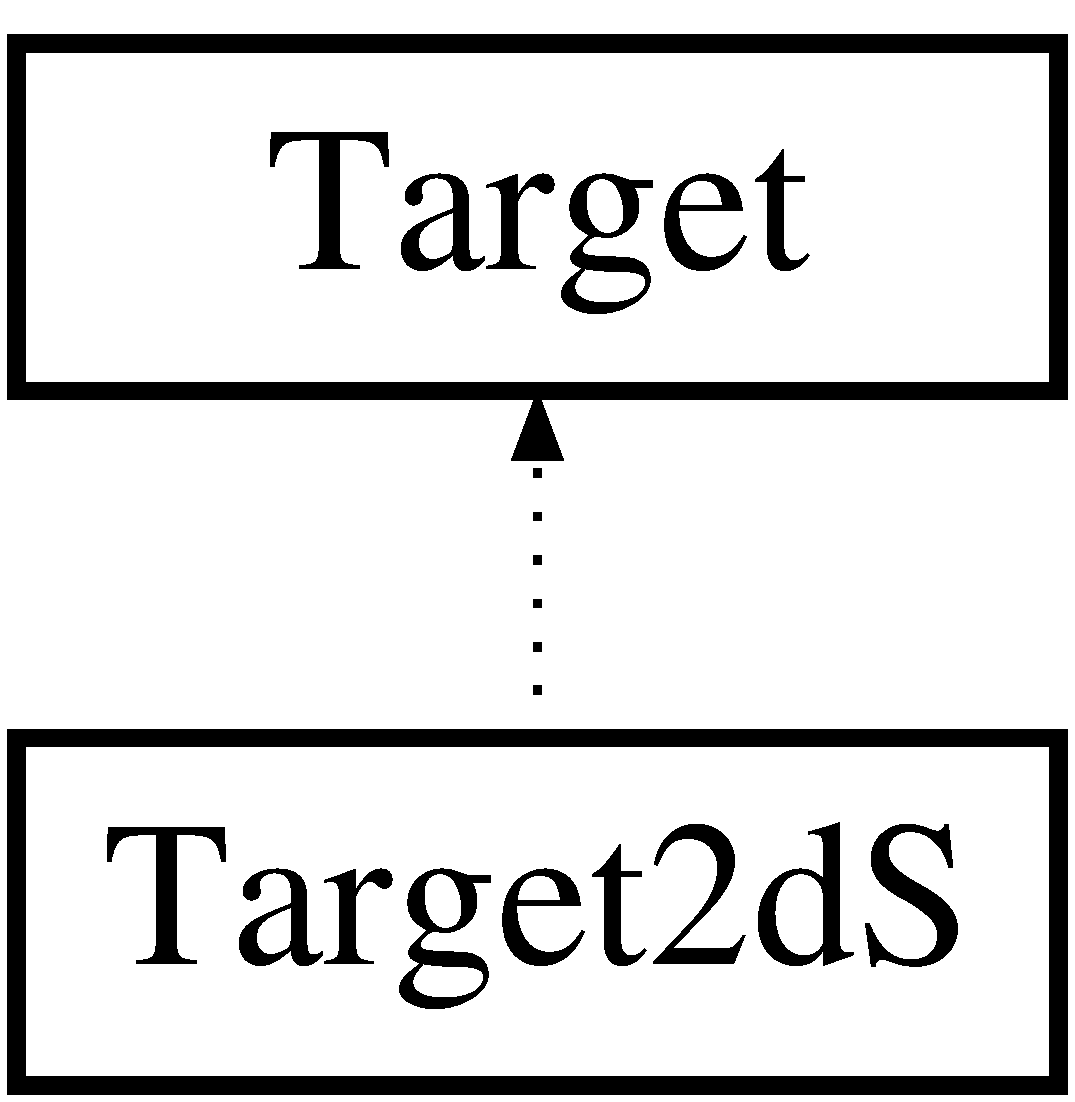
\includegraphics[height=2.000000cm]{class_target2d_s}
\end{center}
\end{figure}


\subsection{Detailed Description}
A sampled 2d target, consist of a collection of samples of the reflectivity function. These samples are used to evaluate teh relfectivity function using some interpolation method. 

Definition at line 27 of file Target.\+h.



The documentation for this class was generated from the following file\+:\begin{DoxyCompactItemize}
\item 
lib/\hyperlink{_target_8h}{Target.\+h}\end{DoxyCompactItemize}

\hypertarget{class_target3d_s}{}\section{Target3dS Class Reference}
\label{class_target3d_s}\index{Target3dS@{Target3dS}}


{\ttfamily \#include $<$Target.\+h$>$}

Inheritance diagram for Target3dS\+:\begin{figure}[H]
\begin{center}
\leavevmode
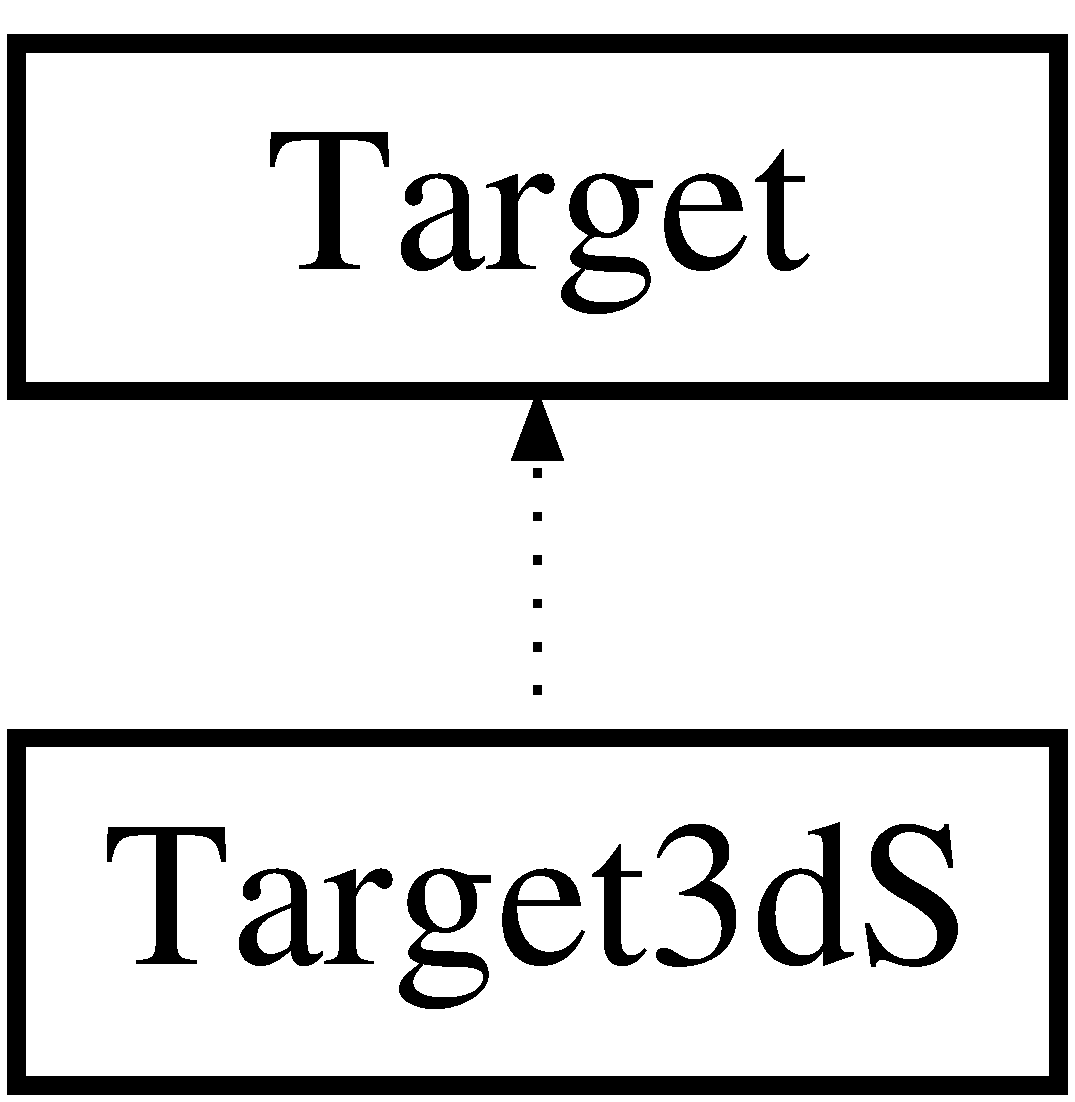
\includegraphics[height=2.000000cm]{class_target3d_s}
\end{center}
\end{figure}


\subsection{Detailed Description}


Definition at line 56 of file Target.\+h.



The documentation for this class was generated from the following file\+:\begin{DoxyCompactItemize}
\item 
lib/\hyperlink{_target_8h}{Target.\+h}\end{DoxyCompactItemize}

\chapter{File Documentation}
\hypertarget{_data___generator_8cpp}{}\section{Data\+\_\+\+Generator/\+Data\+\_\+\+Generator.cpp File Reference}
\label{_data___generator_8cpp}\index{Data\+\_\+\+Generator/\+Data\+\_\+\+Generator.\+cpp@{Data\+\_\+\+Generator/\+Data\+\_\+\+Generator.\+cpp}}
{\ttfamily \#include \char`\"{}Data\+\_\+\+Generator.\+h\char`\"{}}\newline
\subsection*{Functions}
\begin{DoxyCompactItemize}
\item 
int \hyperlink{_data___generator_8cpp_a0ddf1224851353fc92bfbff6f499fa97}{main} (int argc, char $\ast$argv\mbox{[}$\,$\mbox{]})
\end{DoxyCompactItemize}


\subsection{Function Documentation}
\mbox{\Hypertarget{_data___generator_8cpp_a0ddf1224851353fc92bfbff6f499fa97}\label{_data___generator_8cpp_a0ddf1224851353fc92bfbff6f499fa97}} 
\index{Data\+\_\+\+Generator.\+cpp@{Data\+\_\+\+Generator.\+cpp}!main@{main}}
\index{main@{main}!Data\+\_\+\+Generator.\+cpp@{Data\+\_\+\+Generator.\+cpp}}
\subsubsection{\texorpdfstring{main()}{main()}}
{\footnotesize\ttfamily int main (\begin{DoxyParamCaption}\item[{int}]{argc,  }\item[{char $\ast$}]{argv\mbox{[}$\,$\mbox{]} }\end{DoxyParamCaption})}



Definition at line 9 of file Data\+\_\+\+Generator.\+cpp.


\hypertarget{_data___generator_8h}{}\section{Data\+\_\+\+Generator/\+Data\+\_\+\+Generator.h File Reference}
\label{_data___generator_8h}\index{Data\+\_\+\+Generator/\+Data\+\_\+\+Generator.\+h@{Data\+\_\+\+Generator/\+Data\+\_\+\+Generator.\+h}}
\subsection*{Classes}
\begin{DoxyCompactItemize}
\item 
class \hyperlink{class_data_generator}{Data\+Generator}
\item 
class \hyperlink{class_data_generator2d}{Data\+Generator2d}
\end{DoxyCompactItemize}
\subsection*{Functions}
\begin{DoxyCompactItemize}
\item 
const complex$<$ double $>$ \hyperlink{_data___generator_8h_a5d6816662449d5e74ab1f78234044260}{i} (0, 1)
\item 
complex$<$ double $>$ \hyperlink{_data___generator_8h_ad28d23d18460a766bace637017e0ffae}{f} (point y, complex$<$ double $>$ $\ast$d)
\end{DoxyCompactItemize}
\subsection*{Variables}
\begin{DoxyCompactItemize}
\item 
const double \hyperlink{_data___generator_8h_a43016d873124d39034edb8cd164794db}{pi} =3.\+14159265359
\item 
const double \hyperlink{_data___generator_8h_a238dd1656c08db3032dac4e8933ec29f}{c\+\_\+0} =299792458
\item 
const int \hyperlink{_data___generator_8h_ab2b6b0c222cd1ce70d6a831f57241e59}{N} =4
\item 
const int \hyperlink{_data___generator_8h_a9edc6895d567e0ddcdd3cc20df3f3b4b}{M} =\hyperlink{_data___generator_8h_ab2b6b0c222cd1ce70d6a831f57241e59}{N}$\ast$\hyperlink{_data___generator_8h_ab2b6b0c222cd1ce70d6a831f57241e59}{N}
\item 
const int \hyperlink{_data___generator_8h_a7b63ccc35ac484b9f41e37ccd0cb31bd}{K} =1
\item 
const double \hyperlink{_data___generator_8h_a96d9e72424bb3750a125bc08bba688ff}{image\+\_\+height} =0
\item 
\hyperlink{class_data_generator2d}{Data\+Generator2d} \hyperlink{_data___generator_8h_aeb7bb2aca60ddfc3124525269662df7a}{format} =\char`\"{}R\+AW\char`\"{}
\end{DoxyCompactItemize}


\subsection{Function Documentation}
\mbox{\Hypertarget{_data___generator_8h_ad28d23d18460a766bace637017e0ffae}\label{_data___generator_8h_ad28d23d18460a766bace637017e0ffae}} 
\index{Data\+\_\+\+Generator.\+h@{Data\+\_\+\+Generator.\+h}!f@{f}}
\index{f@{f}!Data\+\_\+\+Generator.\+h@{Data\+\_\+\+Generator.\+h}}
\subsubsection{\texorpdfstring{f()}{f()}}
{\footnotesize\ttfamily complex$<$double$>$ f (\begin{DoxyParamCaption}\item[{point}]{y,  }\item[{complex$<$ double $>$ $\ast$}]{d }\end{DoxyParamCaption})}



Definition at line 17 of file Data\+\_\+\+Generator.\+h.

\mbox{\Hypertarget{_data___generator_8h_a5d6816662449d5e74ab1f78234044260}\label{_data___generator_8h_a5d6816662449d5e74ab1f78234044260}} 
\index{Data\+\_\+\+Generator.\+h@{Data\+\_\+\+Generator.\+h}!i@{i}}
\index{i@{i}!Data\+\_\+\+Generator.\+h@{Data\+\_\+\+Generator.\+h}}
\subsubsection{\texorpdfstring{i()}{i()}}
{\footnotesize\ttfamily const complex$<$double$>$ i (\begin{DoxyParamCaption}\item[{0}]{,  }\item[{1}]{ }\end{DoxyParamCaption})}



\subsection{Variable Documentation}
\mbox{\Hypertarget{_data___generator_8h_a238dd1656c08db3032dac4e8933ec29f}\label{_data___generator_8h_a238dd1656c08db3032dac4e8933ec29f}} 
\index{Data\+\_\+\+Generator.\+h@{Data\+\_\+\+Generator.\+h}!c\+\_\+0@{c\+\_\+0}}
\index{c\+\_\+0@{c\+\_\+0}!Data\+\_\+\+Generator.\+h@{Data\+\_\+\+Generator.\+h}}
\subsubsection{\texorpdfstring{c\+\_\+0}{c\_0}}
{\footnotesize\ttfamily const double c\+\_\+0 =299792458}



Definition at line 3 of file Data\+\_\+\+Generator.\+h.

\mbox{\Hypertarget{_data___generator_8h_aeb7bb2aca60ddfc3124525269662df7a}\label{_data___generator_8h_aeb7bb2aca60ddfc3124525269662df7a}} 
\index{Data\+\_\+\+Generator.\+h@{Data\+\_\+\+Generator.\+h}!format@{format}}
\index{format@{format}!Data\+\_\+\+Generator.\+h@{Data\+\_\+\+Generator.\+h}}
\subsubsection{\texorpdfstring{format}{format}}
{\footnotesize\ttfamily  \hyperlink{class_data_generator2d}{Data\+Generator2d} format =\char`\"{}R\+AW\char`\"{}}

The data that we would collect physically. Data may have several dimensions. For example, there are three polarizations, slow time, fast time, flight pass, etc. Data can eithe be representedin frequency domain, or time domain. Typically if data is given in frequency domain, then for each pulse(slowtime bin), The collected data has a windowed Fourier transform aplied to it. This is either done in hardward, digitally. \mbox{\Hypertarget{_data___generator_8h_a96d9e72424bb3750a125bc08bba688ff}\label{_data___generator_8h_a96d9e72424bb3750a125bc08bba688ff}} 
\index{Data\+\_\+\+Generator.\+h@{Data\+\_\+\+Generator.\+h}!image\+\_\+height@{image\+\_\+height}}
\index{image\+\_\+height@{image\+\_\+height}!Data\+\_\+\+Generator.\+h@{Data\+\_\+\+Generator.\+h}}
\subsubsection{\texorpdfstring{image\+\_\+height}{image\_height}}
{\footnotesize\ttfamily const double image\+\_\+height =0}



Definition at line 13 of file Data\+\_\+\+Generator.\+h.

\mbox{\Hypertarget{_data___generator_8h_a7b63ccc35ac484b9f41e37ccd0cb31bd}\label{_data___generator_8h_a7b63ccc35ac484b9f41e37ccd0cb31bd}} 
\index{Data\+\_\+\+Generator.\+h@{Data\+\_\+\+Generator.\+h}!K@{K}}
\index{K@{K}!Data\+\_\+\+Generator.\+h@{Data\+\_\+\+Generator.\+h}}
\subsubsection{\texorpdfstring{K}{K}}
{\footnotesize\ttfamily const int K =1}



Definition at line 11 of file Data\+\_\+\+Generator.\+h.

\mbox{\Hypertarget{_data___generator_8h_a9edc6895d567e0ddcdd3cc20df3f3b4b}\label{_data___generator_8h_a9edc6895d567e0ddcdd3cc20df3f3b4b}} 
\index{Data\+\_\+\+Generator.\+h@{Data\+\_\+\+Generator.\+h}!M@{M}}
\index{M@{M}!Data\+\_\+\+Generator.\+h@{Data\+\_\+\+Generator.\+h}}
\subsubsection{\texorpdfstring{M}{M}}
{\footnotesize\ttfamily const int M =\hyperlink{_data___generator_8h_ab2b6b0c222cd1ce70d6a831f57241e59}{N}$\ast$\hyperlink{_data___generator_8h_ab2b6b0c222cd1ce70d6a831f57241e59}{N}}



Definition at line 7 of file Data\+\_\+\+Generator.\+h.

\mbox{\Hypertarget{_data___generator_8h_ab2b6b0c222cd1ce70d6a831f57241e59}\label{_data___generator_8h_ab2b6b0c222cd1ce70d6a831f57241e59}} 
\index{Data\+\_\+\+Generator.\+h@{Data\+\_\+\+Generator.\+h}!N@{N}}
\index{N@{N}!Data\+\_\+\+Generator.\+h@{Data\+\_\+\+Generator.\+h}}
\subsubsection{\texorpdfstring{N}{N}}
{\footnotesize\ttfamily const int N =4}



Definition at line 6 of file Data\+\_\+\+Generator.\+h.

\mbox{\Hypertarget{_data___generator_8h_a43016d873124d39034edb8cd164794db}\label{_data___generator_8h_a43016d873124d39034edb8cd164794db}} 
\index{Data\+\_\+\+Generator.\+h@{Data\+\_\+\+Generator.\+h}!pi@{pi}}
\index{pi@{pi}!Data\+\_\+\+Generator.\+h@{Data\+\_\+\+Generator.\+h}}
\subsubsection{\texorpdfstring{pi}{pi}}
{\footnotesize\ttfamily const double pi =3.\+14159265359}



Definition at line 2 of file Data\+\_\+\+Generator.\+h.


\hypertarget{_image___recoverer_8cpp}{}\section{Image\+\_\+\+Recovery/\+Image\+\_\+\+Recoverer.cpp File Reference}
\label{_image___recoverer_8cpp}\index{Image\+\_\+\+Recovery/\+Image\+\_\+\+Recoverer.\+cpp@{Image\+\_\+\+Recovery/\+Image\+\_\+\+Recoverer.\+cpp}}
{\ttfamily \#include \char`\"{}image\+\_\+recovery.\+h\char`\"{}}\newline
{\ttfamily \#include \char`\"{}input.\+h\char`\"{}}\newline
\subsection*{Functions}
\begin{DoxyCompactItemize}
\item 
int \hyperlink{_image___recoverer_8cpp_abfa7243bfc915d2f9b1565ea215bbd5c}{main} (int argc=1, char $\ast$filenames\mbox{[}$\,$\mbox{]})
\end{DoxyCompactItemize}


\subsection{Function Documentation}
\mbox{\Hypertarget{_image___recoverer_8cpp_abfa7243bfc915d2f9b1565ea215bbd5c}\label{_image___recoverer_8cpp_abfa7243bfc915d2f9b1565ea215bbd5c}} 
\index{Image\+\_\+\+Recoverer.\+cpp@{Image\+\_\+\+Recoverer.\+cpp}!main@{main}}
\index{main@{main}!Image\+\_\+\+Recoverer.\+cpp@{Image\+\_\+\+Recoverer.\+cpp}}
\subsubsection{\texorpdfstring{main()}{main()}}
{\footnotesize\ttfamily int main (\begin{DoxyParamCaption}\item[{int}]{argc = {\ttfamily 1},  }\item[{char $\ast$}]{filenames\mbox{[}$\,$\mbox{]} }\end{DoxyParamCaption})}



Definition at line 7 of file Image\+\_\+\+Recoverer.\+cpp.


\hypertarget{_image___recoverer_8h}{}\section{Image\+\_\+\+Recovery/\+Image\+\_\+\+Recoverer.h File Reference}
\label{_image___recoverer_8h}\index{Image\+\_\+\+Recovery/\+Image\+\_\+\+Recoverer.\+h@{Image\+\_\+\+Recovery/\+Image\+\_\+\+Recoverer.\+h}}
{\ttfamily \#include $<$complex$>$}\newline
{\ttfamily \#include $<$cstring$>$}\newline
{\ttfamily \#include $<$fstream$>$}\newline
{\ttfamily \#include $<$iostream$>$}\newline
{\ttfamily \#include $<$math.\+h$>$}\newline
{\ttfamily \#include $<$stdlib.\+h$>$}\newline
{\ttfamily \#include $<$string$>$}\newline
\subsection*{Classes}
\begin{DoxyCompactItemize}
\item 
class \hyperlink{class_image_recoverer}{Image\+Recoverer}
\item 
class \hyperlink{class_imaging_plane}{Imaging\+Plane}
\begin{DoxyCompactList}\small\item\em The plane that. \end{DoxyCompactList}\item 
class \hyperlink{class_image_recoverer2d}{Image\+Recoverer2d}
\item 
class \hyperlink{class_image_recoverer3d}{Image\+Recoverer3d}
\end{DoxyCompactItemize}

\hypertarget{_image___recoverer___butterfly_8h}{}\section{Image\+\_\+\+Recovery/\+Image\+\_\+\+Recoverer\+\_\+\+Butterfly.h File Reference}
\label{_image___recoverer___butterfly_8h}\index{Image\+\_\+\+Recovery/\+Image\+\_\+\+Recoverer\+\_\+\+Butterfly.\+h@{Image\+\_\+\+Recovery/\+Image\+\_\+\+Recoverer\+\_\+\+Butterfly.\+h}}

\hypertarget{_image___recoverer___direct_8h}{}\section{Image\+\_\+\+Recovery/\+Image\+\_\+\+Recoverer\+\_\+\+Direct.h File Reference}
\label{_image___recoverer___direct_8h}\index{Image\+\_\+\+Recovery/\+Image\+\_\+\+Recoverer\+\_\+\+Direct.\+h@{Image\+\_\+\+Recovery/\+Image\+\_\+\+Recoverer\+\_\+\+Direct.\+h}}
\subsection*{Classes}
\begin{DoxyCompactItemize}
\item 
class \hyperlink{class_image_recoverer_direct}{Image\+Recoverer\+Direct}
\end{DoxyCompactItemize}
\subsection*{Functions}
\begin{DoxyCompactItemize}
\item 
void \hyperlink{_image___recoverer___direct_8h_a15a2b54cb9d8aa4d5abd90802b1bc34c}{Image\+\_\+\+Recovery\+\_\+\+Direct} (double $\ast$recovered\+\_\+reflectivity, complex$<$ double $>$ $\ast$data, ostream \&log)
\end{DoxyCompactItemize}


\subsection{Function Documentation}
\mbox{\Hypertarget{_image___recoverer___direct_8h_a15a2b54cb9d8aa4d5abd90802b1bc34c}\label{_image___recoverer___direct_8h_a15a2b54cb9d8aa4d5abd90802b1bc34c}} 
\index{Image\+\_\+\+Recoverer\+\_\+\+Direct.\+h@{Image\+\_\+\+Recoverer\+\_\+\+Direct.\+h}!Image\+\_\+\+Recovery\+\_\+\+Direct@{Image\+\_\+\+Recovery\+\_\+\+Direct}}
\index{Image\+\_\+\+Recovery\+\_\+\+Direct@{Image\+\_\+\+Recovery\+\_\+\+Direct}!Image\+\_\+\+Recoverer\+\_\+\+Direct.\+h@{Image\+\_\+\+Recoverer\+\_\+\+Direct.\+h}}
\subsubsection{\texorpdfstring{Image\+\_\+\+Recovery\+\_\+\+Direct()}{Image\_Recovery\_Direct()}}
{\footnotesize\ttfamily void Image\+\_\+\+Recovery\+\_\+\+Direct (\begin{DoxyParamCaption}\item[{double $\ast$}]{recovered\+\_\+reflectivity,  }\item[{complex$<$ double $>$ $\ast$}]{data,  }\item[{ostream \&}]{log }\end{DoxyParamCaption})}



Definition at line 12 of file Image\+\_\+\+Recoverer\+\_\+\+Direct.\+h.


\hypertarget{_math_8h}{}\section{lib/\+Math.h File Reference}
\label{_math_8h}\index{lib/\+Math.\+h@{lib/\+Math.\+h}}
\subsection*{Classes}
\begin{DoxyCompactItemize}
\item 
class \hyperlink{class_math}{Math}
\end{DoxyCompactItemize}
\subsection*{Functions}
\begin{DoxyCompactItemize}
\item 
const complex$<$ double $>$ \hyperlink{_math_8h_a5d6816662449d5e74ab1f78234044260}{i} (0, 1)
\end{DoxyCompactItemize}
\subsection*{Variables}
\begin{DoxyCompactItemize}
\item 
const double \hyperlink{_math_8h_a43016d873124d39034edb8cd164794db}{pi} = 3.\+14159265359
\item 
const double \hyperlink{_math_8h_a238dd1656c08db3032dac4e8933ec29f}{c\+\_\+0} = 299792458
\end{DoxyCompactItemize}


\subsection{Function Documentation}
\mbox{\Hypertarget{_math_8h_a5d6816662449d5e74ab1f78234044260}\label{_math_8h_a5d6816662449d5e74ab1f78234044260}} 
\index{Math.\+h@{Math.\+h}!i@{i}}
\index{i@{i}!Math.\+h@{Math.\+h}}
\subsubsection{\texorpdfstring{i()}{i()}}
{\footnotesize\ttfamily const complex$<$double$>$ i (\begin{DoxyParamCaption}\item[{0}]{,  }\item[{1}]{ }\end{DoxyParamCaption})}



\subsection{Variable Documentation}
\mbox{\Hypertarget{_math_8h_a238dd1656c08db3032dac4e8933ec29f}\label{_math_8h_a238dd1656c08db3032dac4e8933ec29f}} 
\index{Math.\+h@{Math.\+h}!c\+\_\+0@{c\+\_\+0}}
\index{c\+\_\+0@{c\+\_\+0}!Math.\+h@{Math.\+h}}
\subsubsection{\texorpdfstring{c\+\_\+0}{c\_0}}
{\footnotesize\ttfamily const double c\+\_\+0 = 299792458}



Definition at line 3 of file Math.\+h.

\mbox{\Hypertarget{_math_8h_a43016d873124d39034edb8cd164794db}\label{_math_8h_a43016d873124d39034edb8cd164794db}} 
\index{Math.\+h@{Math.\+h}!pi@{pi}}
\index{pi@{pi}!Math.\+h@{Math.\+h}}
\subsubsection{\texorpdfstring{pi}{pi}}
{\footnotesize\ttfamily const double pi = 3.\+14159265359}



Definition at line 2 of file Math.\+h.


\hypertarget{_s_a_r_8h}{}\section{lib/\+S\+AR.h File Reference}
\label{_s_a_r_8h}\index{lib/\+S\+A\+R.\+h@{lib/\+S\+A\+R.\+h}}
\subsection*{Classes}
\begin{DoxyCompactItemize}
\item 
class \hyperlink{class_s_a_r}{S\+AR}
\item 
class \hyperlink{class_signal}{Signal}
\begin{DoxyCompactList}\small\item\em Represents the signal that the antenna will modulate and apply as a current to the. \end{DoxyCompactList}\item 
class \hyperlink{class_chirp}{Chirp}
\item 
class \hyperlink{class_rect}{Rect}
\item 
class \hyperlink{class_antenna}{Antenna}
\end{DoxyCompactItemize}

\hypertarget{_target_8h}{}\section{lib/\+Target.h File Reference}
\label{_target_8h}\index{lib/\+Target.\+h@{lib/\+Target.\+h}}
\subsection*{Classes}
\begin{DoxyCompactItemize}
\item 
class \hyperlink{class_target}{Target}
\item 
class \hyperlink{class_target2d_s}{Target2dS}
\item 
class \hyperlink{class_target3d_s}{Target3dS}
\item 
class \hyperlink{class_target2d_f}{Target2dF}
\end{DoxyCompactItemize}
\subsection*{Functions}
\begin{DoxyCompactItemize}
\item 
complex$<$ double $>$ \hyperlink{_target_8h_ad28d23d18460a766bace637017e0ffae}{f} (point y, complex$<$ double $>$ $\ast$d)
\item 
complex$<$ double $>$ \hyperlink{_target_8h_abe8880126524e4cd8a95094d7e70c4d7}{p} (double w)
\item 
complex$<$ double $>$ \hyperlink{_target_8h_a1518bf2507ae0de796462fe244a92884}{interp} (complex$<$ double $>$ $\ast$d, double sl, double qj)
\item 
double \hyperlink{_target_8h_a748e17292f693395243fe998c44ed79f}{phi} (point x, point y)
\end{DoxyCompactItemize}


\subsection{Function Documentation}
\mbox{\Hypertarget{_target_8h_ad28d23d18460a766bace637017e0ffae}\label{_target_8h_ad28d23d18460a766bace637017e0ffae}} 
\index{Target.\+h@{Target.\+h}!f@{f}}
\index{f@{f}!Target.\+h@{Target.\+h}}
\subsubsection{\texorpdfstring{f()}{f()}}
{\footnotesize\ttfamily complex$<$double$>$ f (\begin{DoxyParamCaption}\item[{point}]{y,  }\item[{complex$<$ double $>$ $\ast$}]{d }\end{DoxyParamCaption})}



Definition at line 17 of file Data\+\_\+\+Generator.\+h.

\mbox{\Hypertarget{_target_8h_a1518bf2507ae0de796462fe244a92884}\label{_target_8h_a1518bf2507ae0de796462fe244a92884}} 
\index{Target.\+h@{Target.\+h}!interp@{interp}}
\index{interp@{interp}!Target.\+h@{Target.\+h}}
\subsubsection{\texorpdfstring{interp()}{interp()}}
{\footnotesize\ttfamily complex$<$double$>$ interp (\begin{DoxyParamCaption}\item[{complex$<$ double $>$ $\ast$}]{d,  }\item[{double}]{sl,  }\item[{double}]{qj }\end{DoxyParamCaption})}

\mbox{\Hypertarget{_target_8h_abe8880126524e4cd8a95094d7e70c4d7}\label{_target_8h_abe8880126524e4cd8a95094d7e70c4d7}} 
\index{Target.\+h@{Target.\+h}!p@{p}}
\index{p@{p}!Target.\+h@{Target.\+h}}
\subsubsection{\texorpdfstring{p()}{p()}}
{\footnotesize\ttfamily complex$<$double$>$ p (\begin{DoxyParamCaption}\item[{double}]{w }\end{DoxyParamCaption})}

\mbox{\Hypertarget{_target_8h_a748e17292f693395243fe998c44ed79f}\label{_target_8h_a748e17292f693395243fe998c44ed79f}} 
\index{Target.\+h@{Target.\+h}!phi@{phi}}
\index{phi@{phi}!Target.\+h@{Target.\+h}}
\subsubsection{\texorpdfstring{phi()}{phi()}}
{\footnotesize\ttfamily double phi (\begin{DoxyParamCaption}\item[{point}]{x,  }\item[{point}]{y }\end{DoxyParamCaption})}


\hypertarget{_r_e_a_d_m_e_8md}{}\section{R\+E\+A\+D\+M\+E.\+md File Reference}
\label{_r_e_a_d_m_e_8md}\index{R\+E\+A\+D\+M\+E.\+md@{R\+E\+A\+D\+M\+E.\+md}}

\hypertarget{_target_creator_8cpp}{}\section{Target\+\_\+\+Generator/\+Target\+Creator.cpp File Reference}
\label{_target_creator_8cpp}\index{Target\+\_\+\+Generator/\+Target\+Creator.\+cpp@{Target\+\_\+\+Generator/\+Target\+Creator.\+cpp}}
{\ttfamily \#include $<$fstream$>$}\newline
{\ttfamily \#include $<$stdio.\+h$>$}\newline
{\ttfamily \#include $<$stdlib.\+h$>$}\newline
{\ttfamily \#include $<$string$>$}\newline
{\ttfamily \#include $<$iostream$>$}\newline
\subsection*{Functions}
\begin{DoxyCompactItemize}
\item 
int \hyperlink{_target_creator_8cpp_a55b340937580925809fddac9d902c4b2}{main} (int arg\+\_\+count, char $\ast$arguments\mbox{[}$\,$\mbox{]})
\end{DoxyCompactItemize}


\subsection{Function Documentation}
\mbox{\Hypertarget{_target_creator_8cpp_a55b340937580925809fddac9d902c4b2}\label{_target_creator_8cpp_a55b340937580925809fddac9d902c4b2}} 
\index{Target\+Creator.\+cpp@{Target\+Creator.\+cpp}!main@{main}}
\index{main@{main}!Target\+Creator.\+cpp@{Target\+Creator.\+cpp}}
\subsubsection{\texorpdfstring{main()}{main()}}
{\footnotesize\ttfamily int main (\begin{DoxyParamCaption}\item[{int}]{arg\+\_\+count,  }\item[{char $\ast$}]{arguments\mbox{[}$\,$\mbox{]} }\end{DoxyParamCaption})}



Definition at line 13 of file Target\+Creator.\+cpp.


\hypertarget{_target_editor_8cpp}{}\section{Target\+\_\+\+Generator/\+Target\+Editor.cpp File Reference}
\label{_target_editor_8cpp}\index{Target\+\_\+\+Generator/\+Target\+Editor.\+cpp@{Target\+\_\+\+Generator/\+Target\+Editor.\+cpp}}

\hypertarget{test_8cpp}{}\section{test/test.cpp File Reference}
\label{test_8cpp}\index{test/test.\+cpp@{test/test.\+cpp}}

\hypertarget{test_8h}{}\section{test/test.h File Reference}
\label{test_8h}\index{test/test.\+h@{test/test.\+h}}
\subsection*{Functions}
\begin{DoxyCompactItemize}
\item 
void \hyperlink{test_8h_a73589c048469dd00a6936e3e928f468b}{Test\+\_\+\+Grid\+\_\+\+Creation} ()
\item 
void \hyperlink{test_8h_a5d9bfe468d0fc4b2738aac8500d2ce2c}{Test\+\_\+\+Indexing} ()
\item 
void \hyperlink{test_8h_a3fe2947dc824985804c88e259460b4f2}{Test\+\_\+\+Image\+\_\+\+Loading} ()
\item 
void \hyperlink{test_8h_a49a3bbfc53d89d60fb40307fa7d32116}{Test\+\_\+\+Data\+\_\+\+Generation} ()
\item 
void \hyperlink{test_8h_a4cadb9c91ab5b36a4d254bb06b4900f3}{Test\+\_\+\+Data\+\_\+\+Loading} ()
\item 
void \hyperlink{test_8h_a7cf248ac1f08fe599358fd5bf302a1ba}{Test\+\_\+\+Image\+\_\+\+Recovery} ()
\item 
void \hyperlink{test_8h_a8e9bfb1e2a0576c20ccc4d5fa4611828}{Test\+\_\+\+Image\+\_\+\+Output} ()
\item 
void \hyperlink{test_8h_a5ca7abf31d308298176441f934aae798}{Print\+\_\+\+Grids} (double $\ast$grids)
\item 
void \hyperlink{test_8h_accdc1d499c43bfea3c07bbcfd7dc3259}{Print\+\_\+\+Weights} (complex$<$ double $>$ $\ast$weights, int l)
\end{DoxyCompactItemize}


\subsection{Function Documentation}
\mbox{\Hypertarget{test_8h_a5ca7abf31d308298176441f934aae798}\label{test_8h_a5ca7abf31d308298176441f934aae798}} 
\index{test.\+h@{test.\+h}!Print\+\_\+\+Grids@{Print\+\_\+\+Grids}}
\index{Print\+\_\+\+Grids@{Print\+\_\+\+Grids}!test.\+h@{test.\+h}}
\subsubsection{\texorpdfstring{Print\+\_\+\+Grids()}{Print\_Grids()}}
{\footnotesize\ttfamily void Print\+\_\+\+Grids (\begin{DoxyParamCaption}\item[{double $\ast$}]{grids }\end{DoxyParamCaption})\hspace{0.3cm}{\ttfamily [inline]}}

\mbox{\Hypertarget{test_8h_accdc1d499c43bfea3c07bbcfd7dc3259}\label{test_8h_accdc1d499c43bfea3c07bbcfd7dc3259}} 
\index{test.\+h@{test.\+h}!Print\+\_\+\+Weights@{Print\+\_\+\+Weights}}
\index{Print\+\_\+\+Weights@{Print\+\_\+\+Weights}!test.\+h@{test.\+h}}
\subsubsection{\texorpdfstring{Print\+\_\+\+Weights()}{Print\_Weights()}}
{\footnotesize\ttfamily void Print\+\_\+\+Weights (\begin{DoxyParamCaption}\item[{complex$<$ double $>$ $\ast$}]{weights,  }\item[{int}]{l }\end{DoxyParamCaption})\hspace{0.3cm}{\ttfamily [inline]}}

\mbox{\Hypertarget{test_8h_a49a3bbfc53d89d60fb40307fa7d32116}\label{test_8h_a49a3bbfc53d89d60fb40307fa7d32116}} 
\index{test.\+h@{test.\+h}!Test\+\_\+\+Data\+\_\+\+Generation@{Test\+\_\+\+Data\+\_\+\+Generation}}
\index{Test\+\_\+\+Data\+\_\+\+Generation@{Test\+\_\+\+Data\+\_\+\+Generation}!test.\+h@{test.\+h}}
\subsubsection{\texorpdfstring{Test\+\_\+\+Data\+\_\+\+Generation()}{Test\_Data\_Generation()}}
{\footnotesize\ttfamily void Test\+\_\+\+Data\+\_\+\+Generation (\begin{DoxyParamCaption}{ }\end{DoxyParamCaption})\hspace{0.3cm}{\ttfamily [inline]}}



Definition at line 103 of file Data\+\_\+\+Generation\+\_\+\+Unit\+\_\+\+Test.\+cpp.

\mbox{\Hypertarget{test_8h_a4cadb9c91ab5b36a4d254bb06b4900f3}\label{test_8h_a4cadb9c91ab5b36a4d254bb06b4900f3}} 
\index{test.\+h@{test.\+h}!Test\+\_\+\+Data\+\_\+\+Loading@{Test\+\_\+\+Data\+\_\+\+Loading}}
\index{Test\+\_\+\+Data\+\_\+\+Loading@{Test\+\_\+\+Data\+\_\+\+Loading}!test.\+h@{test.\+h}}
\subsubsection{\texorpdfstring{Test\+\_\+\+Data\+\_\+\+Loading()}{Test\_Data\_Loading()}}
{\footnotesize\ttfamily void Test\+\_\+\+Data\+\_\+\+Loading (\begin{DoxyParamCaption}{ }\end{DoxyParamCaption})\hspace{0.3cm}{\ttfamily [inline]}}



Definition at line 106 of file Data\+\_\+\+Generation\+\_\+\+Unit\+\_\+\+Test.\+cpp.

\mbox{\Hypertarget{test_8h_a73589c048469dd00a6936e3e928f468b}\label{test_8h_a73589c048469dd00a6936e3e928f468b}} 
\index{test.\+h@{test.\+h}!Test\+\_\+\+Grid\+\_\+\+Creation@{Test\+\_\+\+Grid\+\_\+\+Creation}}
\index{Test\+\_\+\+Grid\+\_\+\+Creation@{Test\+\_\+\+Grid\+\_\+\+Creation}!test.\+h@{test.\+h}}
\subsubsection{\texorpdfstring{Test\+\_\+\+Grid\+\_\+\+Creation()}{Test\_Grid\_Creation()}}
{\footnotesize\ttfamily void Test\+\_\+\+Grid\+\_\+\+Creation (\begin{DoxyParamCaption}{ }\end{DoxyParamCaption})\hspace{0.3cm}{\ttfamily [inline]}}



Definition at line 85 of file Data\+\_\+\+Generation\+\_\+\+Unit\+\_\+\+Test.\+cpp.

\mbox{\Hypertarget{test_8h_a3fe2947dc824985804c88e259460b4f2}\label{test_8h_a3fe2947dc824985804c88e259460b4f2}} 
\index{test.\+h@{test.\+h}!Test\+\_\+\+Image\+\_\+\+Loading@{Test\+\_\+\+Image\+\_\+\+Loading}}
\index{Test\+\_\+\+Image\+\_\+\+Loading@{Test\+\_\+\+Image\+\_\+\+Loading}!test.\+h@{test.\+h}}
\subsubsection{\texorpdfstring{Test\+\_\+\+Image\+\_\+\+Loading()}{Test\_Image\_Loading()}}
{\footnotesize\ttfamily void Test\+\_\+\+Image\+\_\+\+Loading (\begin{DoxyParamCaption}{ }\end{DoxyParamCaption})\hspace{0.3cm}{\ttfamily [inline]}}



Definition at line 99 of file Data\+\_\+\+Generation\+\_\+\+Unit\+\_\+\+Test.\+cpp.

\mbox{\Hypertarget{test_8h_a8e9bfb1e2a0576c20ccc4d5fa4611828}\label{test_8h_a8e9bfb1e2a0576c20ccc4d5fa4611828}} 
\index{test.\+h@{test.\+h}!Test\+\_\+\+Image\+\_\+\+Output@{Test\+\_\+\+Image\+\_\+\+Output}}
\index{Test\+\_\+\+Image\+\_\+\+Output@{Test\+\_\+\+Image\+\_\+\+Output}!test.\+h@{test.\+h}}
\subsubsection{\texorpdfstring{Test\+\_\+\+Image\+\_\+\+Output()}{Test\_Image\_Output()}}
{\footnotesize\ttfamily void Test\+\_\+\+Image\+\_\+\+Output (\begin{DoxyParamCaption}{ }\end{DoxyParamCaption})\hspace{0.3cm}{\ttfamily [inline]}}



Definition at line 112 of file Data\+\_\+\+Generation\+\_\+\+Unit\+\_\+\+Test.\+cpp.

\mbox{\Hypertarget{test_8h_a7cf248ac1f08fe599358fd5bf302a1ba}\label{test_8h_a7cf248ac1f08fe599358fd5bf302a1ba}} 
\index{test.\+h@{test.\+h}!Test\+\_\+\+Image\+\_\+\+Recovery@{Test\+\_\+\+Image\+\_\+\+Recovery}}
\index{Test\+\_\+\+Image\+\_\+\+Recovery@{Test\+\_\+\+Image\+\_\+\+Recovery}!test.\+h@{test.\+h}}
\subsubsection{\texorpdfstring{Test\+\_\+\+Image\+\_\+\+Recovery()}{Test\_Image\_Recovery()}}
{\footnotesize\ttfamily void Test\+\_\+\+Image\+\_\+\+Recovery (\begin{DoxyParamCaption}{ }\end{DoxyParamCaption})\hspace{0.3cm}{\ttfamily [inline]}}



Definition at line 109 of file Data\+\_\+\+Generation\+\_\+\+Unit\+\_\+\+Test.\+cpp.

\mbox{\Hypertarget{test_8h_a5d9bfe468d0fc4b2738aac8500d2ce2c}\label{test_8h_a5d9bfe468d0fc4b2738aac8500d2ce2c}} 
\index{test.\+h@{test.\+h}!Test\+\_\+\+Indexing@{Test\+\_\+\+Indexing}}
\index{Test\+\_\+\+Indexing@{Test\+\_\+\+Indexing}!test.\+h@{test.\+h}}
\subsubsection{\texorpdfstring{Test\+\_\+\+Indexing()}{Test\_Indexing()}}
{\footnotesize\ttfamily void Test\+\_\+\+Indexing (\begin{DoxyParamCaption}{ }\end{DoxyParamCaption})\hspace{0.3cm}{\ttfamily [inline]}}


\hypertarget{_data___generation___unit___test_8cpp}{}\section{Testing/\+Data\+\_\+\+Generation\+\_\+\+Unit\+\_\+\+Test.cpp File Reference}
\label{_data___generation___unit___test_8cpp}\index{Testing/\+Data\+\_\+\+Generation\+\_\+\+Unit\+\_\+\+Test.\+cpp@{Testing/\+Data\+\_\+\+Generation\+\_\+\+Unit\+\_\+\+Test.\+cpp}}
{\ttfamily \#include \char`\"{}input.\+h\char`\"{}}\newline
{\ttfamily \#include \char`\"{}data\+\_\+generation.\+h\char`\"{}}\newline
{\ttfamily \#include \char`\"{}image\+\_\+recovery.\+h\char`\"{}}\newline
{\ttfamily \#include $<$ofstream$>$}\newline
\subsection*{Functions}
\begin{DoxyCompactItemize}
\item 
double \hyperlink{_data___generation___unit___test_8cpp_afeeb58172d4ef5dd2676c4cb3a5bea08}{phi} (double x1, double x2, double y1, double y2)
\item 
double \hyperlink{_data___generation___unit___test_8cpp_a2bc9dab971e913c166e1f9f5597971ae}{f} (double y1, double y2)
\item 
double \hyperlink{_data___generation___unit___test_8cpp_aeeb95c8189127d214acd24fa3720e9d2}{psi} (double x1, double x2, double y1, double y2)
\item 
int \hyperlink{_data___generation___unit___test_8cpp_a0ddf1224851353fc92bfbff6f499fa97}{main} (int argc, char $\ast$argv\mbox{[}$\,$\mbox{]})
\item 
void \hyperlink{_data___generation___unit___test_8cpp_a6aea2ec580dabdeff7cb3738f95dc4c8}{Output\+\_\+\+Weights} (ostream os, complex$<$ double $>$ $\ast$weights, int l)
\item 
void \hyperlink{_data___generation___unit___test_8cpp_ab005e77c7f55f8dcff07ec0f194c98aa}{Output\+\_\+\+Grids} (ostream os, double $\ast$grids)
\item 
void \hyperlink{_data___generation___unit___test_8cpp_a73589c048469dd00a6936e3e928f468b}{Test\+\_\+\+Grid\+\_\+\+Creation} ()
\item 
void \hyperlink{_data___generation___unit___test_8cpp_a1a74da74eecf3f12abcf0d623a67f31f}{Test\+\_\+\+Indexing} (ofstream log)
\item 
void \hyperlink{_data___generation___unit___test_8cpp_a3fe2947dc824985804c88e259460b4f2}{Test\+\_\+\+Image\+\_\+\+Loading} ()
\item 
void \hyperlink{_data___generation___unit___test_8cpp_a49a3bbfc53d89d60fb40307fa7d32116}{Test\+\_\+\+Data\+\_\+\+Generation} ()
\item 
void \hyperlink{_data___generation___unit___test_8cpp_a4cadb9c91ab5b36a4d254bb06b4900f3}{Test\+\_\+\+Data\+\_\+\+Loading} ()
\item 
void \hyperlink{_data___generation___unit___test_8cpp_a7cf248ac1f08fe599358fd5bf302a1ba}{Test\+\_\+\+Image\+\_\+\+Recovery} ()
\item 
void \hyperlink{_data___generation___unit___test_8cpp_a8e9bfb1e2a0576c20ccc4d5fa4611828}{Test\+\_\+\+Image\+\_\+\+Output} ()
\item 
void \hyperlink{_data___generation___unit___test_8cpp_a4823f2cf4868a5b06871f204aba71a53}{Test\+\_\+\+Chebyshev\+\_\+\+Interpolation} ()
\end{DoxyCompactItemize}


\subsection{Function Documentation}
\mbox{\Hypertarget{_data___generation___unit___test_8cpp_a2bc9dab971e913c166e1f9f5597971ae}\label{_data___generation___unit___test_8cpp_a2bc9dab971e913c166e1f9f5597971ae}} 
\index{Data\+\_\+\+Generation\+\_\+\+Unit\+\_\+\+Test.\+cpp@{Data\+\_\+\+Generation\+\_\+\+Unit\+\_\+\+Test.\+cpp}!f@{f}}
\index{f@{f}!Data\+\_\+\+Generation\+\_\+\+Unit\+\_\+\+Test.\+cpp@{Data\+\_\+\+Generation\+\_\+\+Unit\+\_\+\+Test.\+cpp}}
\subsubsection{\texorpdfstring{f()}{f()}}
{\footnotesize\ttfamily double f (\begin{DoxyParamCaption}\item[{double}]{y1,  }\item[{double}]{y2 }\end{DoxyParamCaption})}

\mbox{\Hypertarget{_data___generation___unit___test_8cpp_a0ddf1224851353fc92bfbff6f499fa97}\label{_data___generation___unit___test_8cpp_a0ddf1224851353fc92bfbff6f499fa97}} 
\index{Data\+\_\+\+Generation\+\_\+\+Unit\+\_\+\+Test.\+cpp@{Data\+\_\+\+Generation\+\_\+\+Unit\+\_\+\+Test.\+cpp}!main@{main}}
\index{main@{main}!Data\+\_\+\+Generation\+\_\+\+Unit\+\_\+\+Test.\+cpp@{Data\+\_\+\+Generation\+\_\+\+Unit\+\_\+\+Test.\+cpp}}
\subsubsection{\texorpdfstring{main()}{main()}}
{\footnotesize\ttfamily int main (\begin{DoxyParamCaption}\item[{int}]{argc,  }\item[{char $\ast$}]{argv\mbox{[}$\,$\mbox{]} }\end{DoxyParamCaption})}

\hyperlink{_data___generation___unit___test_8cpp_a8e9bfb1e2a0576c20ccc4d5fa4611828}{Test\+\_\+\+Image\+\_\+\+Output()}; 

Definition at line 15 of file Data\+\_\+\+Generation\+\_\+\+Unit\+\_\+\+Test.\+cpp.

\mbox{\Hypertarget{_data___generation___unit___test_8cpp_ab005e77c7f55f8dcff07ec0f194c98aa}\label{_data___generation___unit___test_8cpp_ab005e77c7f55f8dcff07ec0f194c98aa}} 
\index{Data\+\_\+\+Generation\+\_\+\+Unit\+\_\+\+Test.\+cpp@{Data\+\_\+\+Generation\+\_\+\+Unit\+\_\+\+Test.\+cpp}!Output\+\_\+\+Grids@{Output\+\_\+\+Grids}}
\index{Output\+\_\+\+Grids@{Output\+\_\+\+Grids}!Data\+\_\+\+Generation\+\_\+\+Unit\+\_\+\+Test.\+cpp@{Data\+\_\+\+Generation\+\_\+\+Unit\+\_\+\+Test.\+cpp}}
\subsubsection{\texorpdfstring{Output\+\_\+\+Grids()}{Output\_Grids()}}
{\footnotesize\ttfamily void Output\+\_\+\+Grids (\begin{DoxyParamCaption}\item[{ostream}]{os,  }\item[{double $\ast$}]{grids }\end{DoxyParamCaption})\hspace{0.3cm}{\ttfamily [inline]}}



Definition at line 68 of file Data\+\_\+\+Generation\+\_\+\+Unit\+\_\+\+Test.\+cpp.

\mbox{\Hypertarget{_data___generation___unit___test_8cpp_a6aea2ec580dabdeff7cb3738f95dc4c8}\label{_data___generation___unit___test_8cpp_a6aea2ec580dabdeff7cb3738f95dc4c8}} 
\index{Data\+\_\+\+Generation\+\_\+\+Unit\+\_\+\+Test.\+cpp@{Data\+\_\+\+Generation\+\_\+\+Unit\+\_\+\+Test.\+cpp}!Output\+\_\+\+Weights@{Output\+\_\+\+Weights}}
\index{Output\+\_\+\+Weights@{Output\+\_\+\+Weights}!Data\+\_\+\+Generation\+\_\+\+Unit\+\_\+\+Test.\+cpp@{Data\+\_\+\+Generation\+\_\+\+Unit\+\_\+\+Test.\+cpp}}
\subsubsection{\texorpdfstring{Output\+\_\+\+Weights()}{Output\_Weights()}}
{\footnotesize\ttfamily void Output\+\_\+\+Weights (\begin{DoxyParamCaption}\item[{ostream}]{os,  }\item[{complex$<$ double $>$ $\ast$}]{weights,  }\item[{int}]{l }\end{DoxyParamCaption})\hspace{0.3cm}{\ttfamily [inline]}}



Definition at line 56 of file Data\+\_\+\+Generation\+\_\+\+Unit\+\_\+\+Test.\+cpp.

\mbox{\Hypertarget{_data___generation___unit___test_8cpp_afeeb58172d4ef5dd2676c4cb3a5bea08}\label{_data___generation___unit___test_8cpp_afeeb58172d4ef5dd2676c4cb3a5bea08}} 
\index{Data\+\_\+\+Generation\+\_\+\+Unit\+\_\+\+Test.\+cpp@{Data\+\_\+\+Generation\+\_\+\+Unit\+\_\+\+Test.\+cpp}!phi@{phi}}
\index{phi@{phi}!Data\+\_\+\+Generation\+\_\+\+Unit\+\_\+\+Test.\+cpp@{Data\+\_\+\+Generation\+\_\+\+Unit\+\_\+\+Test.\+cpp}}
\subsubsection{\texorpdfstring{phi()}{phi()}}
{\footnotesize\ttfamily double phi (\begin{DoxyParamCaption}\item[{double}]{x1,  }\item[{double}]{x2,  }\item[{double}]{y1,  }\item[{double}]{y2 }\end{DoxyParamCaption})}

\mbox{\Hypertarget{_data___generation___unit___test_8cpp_aeeb95c8189127d214acd24fa3720e9d2}\label{_data___generation___unit___test_8cpp_aeeb95c8189127d214acd24fa3720e9d2}} 
\index{Data\+\_\+\+Generation\+\_\+\+Unit\+\_\+\+Test.\+cpp@{Data\+\_\+\+Generation\+\_\+\+Unit\+\_\+\+Test.\+cpp}!psi@{psi}}
\index{psi@{psi}!Data\+\_\+\+Generation\+\_\+\+Unit\+\_\+\+Test.\+cpp@{Data\+\_\+\+Generation\+\_\+\+Unit\+\_\+\+Test.\+cpp}}
\subsubsection{\texorpdfstring{psi()}{psi()}}
{\footnotesize\ttfamily double psi (\begin{DoxyParamCaption}\item[{double}]{x1,  }\item[{double}]{x2,  }\item[{double}]{y1,  }\item[{double}]{y2 }\end{DoxyParamCaption})}

\mbox{\Hypertarget{_data___generation___unit___test_8cpp_a4823f2cf4868a5b06871f204aba71a53}\label{_data___generation___unit___test_8cpp_a4823f2cf4868a5b06871f204aba71a53}} 
\index{Data\+\_\+\+Generation\+\_\+\+Unit\+\_\+\+Test.\+cpp@{Data\+\_\+\+Generation\+\_\+\+Unit\+\_\+\+Test.\+cpp}!Test\+\_\+\+Chebyshev\+\_\+\+Interpolation@{Test\+\_\+\+Chebyshev\+\_\+\+Interpolation}}
\index{Test\+\_\+\+Chebyshev\+\_\+\+Interpolation@{Test\+\_\+\+Chebyshev\+\_\+\+Interpolation}!Data\+\_\+\+Generation\+\_\+\+Unit\+\_\+\+Test.\+cpp@{Data\+\_\+\+Generation\+\_\+\+Unit\+\_\+\+Test.\+cpp}}
\subsubsection{\texorpdfstring{Test\+\_\+\+Chebyshev\+\_\+\+Interpolation()}{Test\_Chebyshev\_Interpolation()}}
{\footnotesize\ttfamily void Test\+\_\+\+Chebyshev\+\_\+\+Interpolation (\begin{DoxyParamCaption}{ }\end{DoxyParamCaption})\hspace{0.3cm}{\ttfamily [inline]}}



Definition at line 117 of file Data\+\_\+\+Generation\+\_\+\+Unit\+\_\+\+Test.\+cpp.

\mbox{\Hypertarget{_data___generation___unit___test_8cpp_a49a3bbfc53d89d60fb40307fa7d32116}\label{_data___generation___unit___test_8cpp_a49a3bbfc53d89d60fb40307fa7d32116}} 
\index{Data\+\_\+\+Generation\+\_\+\+Unit\+\_\+\+Test.\+cpp@{Data\+\_\+\+Generation\+\_\+\+Unit\+\_\+\+Test.\+cpp}!Test\+\_\+\+Data\+\_\+\+Generation@{Test\+\_\+\+Data\+\_\+\+Generation}}
\index{Test\+\_\+\+Data\+\_\+\+Generation@{Test\+\_\+\+Data\+\_\+\+Generation}!Data\+\_\+\+Generation\+\_\+\+Unit\+\_\+\+Test.\+cpp@{Data\+\_\+\+Generation\+\_\+\+Unit\+\_\+\+Test.\+cpp}}
\subsubsection{\texorpdfstring{Test\+\_\+\+Data\+\_\+\+Generation()}{Test\_Data\_Generation()}}
{\footnotesize\ttfamily void Test\+\_\+\+Data\+\_\+\+Generation (\begin{DoxyParamCaption}{ }\end{DoxyParamCaption})\hspace{0.3cm}{\ttfamily [inline]}}



Definition at line 103 of file Data\+\_\+\+Generation\+\_\+\+Unit\+\_\+\+Test.\+cpp.

\mbox{\Hypertarget{_data___generation___unit___test_8cpp_a4cadb9c91ab5b36a4d254bb06b4900f3}\label{_data___generation___unit___test_8cpp_a4cadb9c91ab5b36a4d254bb06b4900f3}} 
\index{Data\+\_\+\+Generation\+\_\+\+Unit\+\_\+\+Test.\+cpp@{Data\+\_\+\+Generation\+\_\+\+Unit\+\_\+\+Test.\+cpp}!Test\+\_\+\+Data\+\_\+\+Loading@{Test\+\_\+\+Data\+\_\+\+Loading}}
\index{Test\+\_\+\+Data\+\_\+\+Loading@{Test\+\_\+\+Data\+\_\+\+Loading}!Data\+\_\+\+Generation\+\_\+\+Unit\+\_\+\+Test.\+cpp@{Data\+\_\+\+Generation\+\_\+\+Unit\+\_\+\+Test.\+cpp}}
\subsubsection{\texorpdfstring{Test\+\_\+\+Data\+\_\+\+Loading()}{Test\_Data\_Loading()}}
{\footnotesize\ttfamily void Test\+\_\+\+Data\+\_\+\+Loading (\begin{DoxyParamCaption}{ }\end{DoxyParamCaption})\hspace{0.3cm}{\ttfamily [inline]}}



Definition at line 106 of file Data\+\_\+\+Generation\+\_\+\+Unit\+\_\+\+Test.\+cpp.

\mbox{\Hypertarget{_data___generation___unit___test_8cpp_a73589c048469dd00a6936e3e928f468b}\label{_data___generation___unit___test_8cpp_a73589c048469dd00a6936e3e928f468b}} 
\index{Data\+\_\+\+Generation\+\_\+\+Unit\+\_\+\+Test.\+cpp@{Data\+\_\+\+Generation\+\_\+\+Unit\+\_\+\+Test.\+cpp}!Test\+\_\+\+Grid\+\_\+\+Creation@{Test\+\_\+\+Grid\+\_\+\+Creation}}
\index{Test\+\_\+\+Grid\+\_\+\+Creation@{Test\+\_\+\+Grid\+\_\+\+Creation}!Data\+\_\+\+Generation\+\_\+\+Unit\+\_\+\+Test.\+cpp@{Data\+\_\+\+Generation\+\_\+\+Unit\+\_\+\+Test.\+cpp}}
\subsubsection{\texorpdfstring{Test\+\_\+\+Grid\+\_\+\+Creation()}{Test\_Grid\_Creation()}}
{\footnotesize\ttfamily void Test\+\_\+\+Grid\+\_\+\+Creation (\begin{DoxyParamCaption}{ }\end{DoxyParamCaption})\hspace{0.3cm}{\ttfamily [inline]}}



Definition at line 85 of file Data\+\_\+\+Generation\+\_\+\+Unit\+\_\+\+Test.\+cpp.

\mbox{\Hypertarget{_data___generation___unit___test_8cpp_a3fe2947dc824985804c88e259460b4f2}\label{_data___generation___unit___test_8cpp_a3fe2947dc824985804c88e259460b4f2}} 
\index{Data\+\_\+\+Generation\+\_\+\+Unit\+\_\+\+Test.\+cpp@{Data\+\_\+\+Generation\+\_\+\+Unit\+\_\+\+Test.\+cpp}!Test\+\_\+\+Image\+\_\+\+Loading@{Test\+\_\+\+Image\+\_\+\+Loading}}
\index{Test\+\_\+\+Image\+\_\+\+Loading@{Test\+\_\+\+Image\+\_\+\+Loading}!Data\+\_\+\+Generation\+\_\+\+Unit\+\_\+\+Test.\+cpp@{Data\+\_\+\+Generation\+\_\+\+Unit\+\_\+\+Test.\+cpp}}
\subsubsection{\texorpdfstring{Test\+\_\+\+Image\+\_\+\+Loading()}{Test\_Image\_Loading()}}
{\footnotesize\ttfamily void Test\+\_\+\+Image\+\_\+\+Loading (\begin{DoxyParamCaption}{ }\end{DoxyParamCaption})\hspace{0.3cm}{\ttfamily [inline]}}



Definition at line 99 of file Data\+\_\+\+Generation\+\_\+\+Unit\+\_\+\+Test.\+cpp.

\mbox{\Hypertarget{_data___generation___unit___test_8cpp_a8e9bfb1e2a0576c20ccc4d5fa4611828}\label{_data___generation___unit___test_8cpp_a8e9bfb1e2a0576c20ccc4d5fa4611828}} 
\index{Data\+\_\+\+Generation\+\_\+\+Unit\+\_\+\+Test.\+cpp@{Data\+\_\+\+Generation\+\_\+\+Unit\+\_\+\+Test.\+cpp}!Test\+\_\+\+Image\+\_\+\+Output@{Test\+\_\+\+Image\+\_\+\+Output}}
\index{Test\+\_\+\+Image\+\_\+\+Output@{Test\+\_\+\+Image\+\_\+\+Output}!Data\+\_\+\+Generation\+\_\+\+Unit\+\_\+\+Test.\+cpp@{Data\+\_\+\+Generation\+\_\+\+Unit\+\_\+\+Test.\+cpp}}
\subsubsection{\texorpdfstring{Test\+\_\+\+Image\+\_\+\+Output()}{Test\_Image\_Output()}}
{\footnotesize\ttfamily void Test\+\_\+\+Image\+\_\+\+Output (\begin{DoxyParamCaption}{ }\end{DoxyParamCaption})\hspace{0.3cm}{\ttfamily [inline]}}



Definition at line 112 of file Data\+\_\+\+Generation\+\_\+\+Unit\+\_\+\+Test.\+cpp.

\mbox{\Hypertarget{_data___generation___unit___test_8cpp_a7cf248ac1f08fe599358fd5bf302a1ba}\label{_data___generation___unit___test_8cpp_a7cf248ac1f08fe599358fd5bf302a1ba}} 
\index{Data\+\_\+\+Generation\+\_\+\+Unit\+\_\+\+Test.\+cpp@{Data\+\_\+\+Generation\+\_\+\+Unit\+\_\+\+Test.\+cpp}!Test\+\_\+\+Image\+\_\+\+Recovery@{Test\+\_\+\+Image\+\_\+\+Recovery}}
\index{Test\+\_\+\+Image\+\_\+\+Recovery@{Test\+\_\+\+Image\+\_\+\+Recovery}!Data\+\_\+\+Generation\+\_\+\+Unit\+\_\+\+Test.\+cpp@{Data\+\_\+\+Generation\+\_\+\+Unit\+\_\+\+Test.\+cpp}}
\subsubsection{\texorpdfstring{Test\+\_\+\+Image\+\_\+\+Recovery()}{Test\_Image\_Recovery()}}
{\footnotesize\ttfamily void Test\+\_\+\+Image\+\_\+\+Recovery (\begin{DoxyParamCaption}{ }\end{DoxyParamCaption})\hspace{0.3cm}{\ttfamily [inline]}}



Definition at line 109 of file Data\+\_\+\+Generation\+\_\+\+Unit\+\_\+\+Test.\+cpp.

\mbox{\Hypertarget{_data___generation___unit___test_8cpp_a1a74da74eecf3f12abcf0d623a67f31f}\label{_data___generation___unit___test_8cpp_a1a74da74eecf3f12abcf0d623a67f31f}} 
\index{Data\+\_\+\+Generation\+\_\+\+Unit\+\_\+\+Test.\+cpp@{Data\+\_\+\+Generation\+\_\+\+Unit\+\_\+\+Test.\+cpp}!Test\+\_\+\+Indexing@{Test\+\_\+\+Indexing}}
\index{Test\+\_\+\+Indexing@{Test\+\_\+\+Indexing}!Data\+\_\+\+Generation\+\_\+\+Unit\+\_\+\+Test.\+cpp@{Data\+\_\+\+Generation\+\_\+\+Unit\+\_\+\+Test.\+cpp}}
\subsubsection{\texorpdfstring{Test\+\_\+\+Indexing()}{Test\_Indexing()}}
{\footnotesize\ttfamily void Test\+\_\+\+Indexing (\begin{DoxyParamCaption}\item[{ofstream}]{log }\end{DoxyParamCaption})\hspace{0.3cm}{\ttfamily [inline]}}



Definition at line 93 of file Data\+\_\+\+Generation\+\_\+\+Unit\+\_\+\+Test.\+cpp.


\hypertarget{_image___editor___unit___test_8cpp}{}\section{Testing/\+Image\+\_\+\+Editor\+\_\+\+Unit\+\_\+\+Test.cpp File Reference}
\label{_image___editor___unit___test_8cpp}\index{Testing/\+Image\+\_\+\+Editor\+\_\+\+Unit\+\_\+\+Test.\+cpp@{Testing/\+Image\+\_\+\+Editor\+\_\+\+Unit\+\_\+\+Test.\+cpp}}
{\ttfamily \#include \char`\"{}input.\+h\char`\"{}}\newline
{\ttfamily \#include \char`\"{}data\+\_\+generation.\+h\char`\"{}}\newline
{\ttfamily \#include \char`\"{}image\+\_\+recovery.\+h\char`\"{}}\newline
{\ttfamily \#include $<$ofstream$>$}\newline
\subsection*{Functions}
\begin{DoxyCompactItemize}
\item 
double \hyperlink{_image___editor___unit___test_8cpp_afeeb58172d4ef5dd2676c4cb3a5bea08}{phi} (double x1, double x2, double y1, double y2)
\item 
double \hyperlink{_image___editor___unit___test_8cpp_a2bc9dab971e913c166e1f9f5597971ae}{f} (double y1, double y2)
\item 
double \hyperlink{_image___editor___unit___test_8cpp_aeeb95c8189127d214acd24fa3720e9d2}{psi} (double x1, double x2, double y1, double y2)
\item 
int \hyperlink{_image___editor___unit___test_8cpp_a0ddf1224851353fc92bfbff6f499fa97}{main} (int argc, char $\ast$argv\mbox{[}$\,$\mbox{]})
\item 
void \hyperlink{_image___editor___unit___test_8cpp_a6aea2ec580dabdeff7cb3738f95dc4c8}{Output\+\_\+\+Weights} (ostream os, complex$<$ double $>$ $\ast$weights, int l)
\item 
void \hyperlink{_image___editor___unit___test_8cpp_ab005e77c7f55f8dcff07ec0f194c98aa}{Output\+\_\+\+Grids} (ostream os, double $\ast$grids)
\item 
void \hyperlink{_image___editor___unit___test_8cpp_a73589c048469dd00a6936e3e928f468b}{Test\+\_\+\+Grid\+\_\+\+Creation} ()
\item 
void \hyperlink{_image___editor___unit___test_8cpp_a1a74da74eecf3f12abcf0d623a67f31f}{Test\+\_\+\+Indexing} (ofstream log)
\item 
void \hyperlink{_image___editor___unit___test_8cpp_a3fe2947dc824985804c88e259460b4f2}{Test\+\_\+\+Image\+\_\+\+Loading} ()
\item 
void \hyperlink{_image___editor___unit___test_8cpp_a49a3bbfc53d89d60fb40307fa7d32116}{Test\+\_\+\+Data\+\_\+\+Generation} ()
\item 
void \hyperlink{_image___editor___unit___test_8cpp_a4cadb9c91ab5b36a4d254bb06b4900f3}{Test\+\_\+\+Data\+\_\+\+Loading} ()
\item 
void \hyperlink{_image___editor___unit___test_8cpp_a7cf248ac1f08fe599358fd5bf302a1ba}{Test\+\_\+\+Image\+\_\+\+Recovery} ()
\item 
void \hyperlink{_image___editor___unit___test_8cpp_a8e9bfb1e2a0576c20ccc4d5fa4611828}{Test\+\_\+\+Image\+\_\+\+Output} ()
\item 
void \hyperlink{_image___editor___unit___test_8cpp_a4823f2cf4868a5b06871f204aba71a53}{Test\+\_\+\+Chebyshev\+\_\+\+Interpolation} ()
\end{DoxyCompactItemize}


\subsection{Function Documentation}
\mbox{\Hypertarget{_image___editor___unit___test_8cpp_a2bc9dab971e913c166e1f9f5597971ae}\label{_image___editor___unit___test_8cpp_a2bc9dab971e913c166e1f9f5597971ae}} 
\index{Image\+\_\+\+Editor\+\_\+\+Unit\+\_\+\+Test.\+cpp@{Image\+\_\+\+Editor\+\_\+\+Unit\+\_\+\+Test.\+cpp}!f@{f}}
\index{f@{f}!Image\+\_\+\+Editor\+\_\+\+Unit\+\_\+\+Test.\+cpp@{Image\+\_\+\+Editor\+\_\+\+Unit\+\_\+\+Test.\+cpp}}
\subsubsection{\texorpdfstring{f()}{f()}}
{\footnotesize\ttfamily double f (\begin{DoxyParamCaption}\item[{double}]{y1,  }\item[{double}]{y2 }\end{DoxyParamCaption})}

\mbox{\Hypertarget{_image___editor___unit___test_8cpp_a0ddf1224851353fc92bfbff6f499fa97}\label{_image___editor___unit___test_8cpp_a0ddf1224851353fc92bfbff6f499fa97}} 
\index{Image\+\_\+\+Editor\+\_\+\+Unit\+\_\+\+Test.\+cpp@{Image\+\_\+\+Editor\+\_\+\+Unit\+\_\+\+Test.\+cpp}!main@{main}}
\index{main@{main}!Image\+\_\+\+Editor\+\_\+\+Unit\+\_\+\+Test.\+cpp@{Image\+\_\+\+Editor\+\_\+\+Unit\+\_\+\+Test.\+cpp}}
\subsubsection{\texorpdfstring{main()}{main()}}
{\footnotesize\ttfamily int main (\begin{DoxyParamCaption}\item[{int}]{argc,  }\item[{char $\ast$}]{argv\mbox{[}$\,$\mbox{]} }\end{DoxyParamCaption})}

\hyperlink{_image___editor___unit___test_8cpp_a8e9bfb1e2a0576c20ccc4d5fa4611828}{Test\+\_\+\+Image\+\_\+\+Output()}; 

Definition at line 15 of file Image\+\_\+\+Editor\+\_\+\+Unit\+\_\+\+Test.\+cpp.

\mbox{\Hypertarget{_image___editor___unit___test_8cpp_ab005e77c7f55f8dcff07ec0f194c98aa}\label{_image___editor___unit___test_8cpp_ab005e77c7f55f8dcff07ec0f194c98aa}} 
\index{Image\+\_\+\+Editor\+\_\+\+Unit\+\_\+\+Test.\+cpp@{Image\+\_\+\+Editor\+\_\+\+Unit\+\_\+\+Test.\+cpp}!Output\+\_\+\+Grids@{Output\+\_\+\+Grids}}
\index{Output\+\_\+\+Grids@{Output\+\_\+\+Grids}!Image\+\_\+\+Editor\+\_\+\+Unit\+\_\+\+Test.\+cpp@{Image\+\_\+\+Editor\+\_\+\+Unit\+\_\+\+Test.\+cpp}}
\subsubsection{\texorpdfstring{Output\+\_\+\+Grids()}{Output\_Grids()}}
{\footnotesize\ttfamily void Output\+\_\+\+Grids (\begin{DoxyParamCaption}\item[{ostream}]{os,  }\item[{double $\ast$}]{grids }\end{DoxyParamCaption})\hspace{0.3cm}{\ttfamily [inline]}}



Definition at line 68 of file Image\+\_\+\+Editor\+\_\+\+Unit\+\_\+\+Test.\+cpp.

\mbox{\Hypertarget{_image___editor___unit___test_8cpp_a6aea2ec580dabdeff7cb3738f95dc4c8}\label{_image___editor___unit___test_8cpp_a6aea2ec580dabdeff7cb3738f95dc4c8}} 
\index{Image\+\_\+\+Editor\+\_\+\+Unit\+\_\+\+Test.\+cpp@{Image\+\_\+\+Editor\+\_\+\+Unit\+\_\+\+Test.\+cpp}!Output\+\_\+\+Weights@{Output\+\_\+\+Weights}}
\index{Output\+\_\+\+Weights@{Output\+\_\+\+Weights}!Image\+\_\+\+Editor\+\_\+\+Unit\+\_\+\+Test.\+cpp@{Image\+\_\+\+Editor\+\_\+\+Unit\+\_\+\+Test.\+cpp}}
\subsubsection{\texorpdfstring{Output\+\_\+\+Weights()}{Output\_Weights()}}
{\footnotesize\ttfamily void Output\+\_\+\+Weights (\begin{DoxyParamCaption}\item[{ostream}]{os,  }\item[{complex$<$ double $>$ $\ast$}]{weights,  }\item[{int}]{l }\end{DoxyParamCaption})\hspace{0.3cm}{\ttfamily [inline]}}



Definition at line 56 of file Image\+\_\+\+Editor\+\_\+\+Unit\+\_\+\+Test.\+cpp.

\mbox{\Hypertarget{_image___editor___unit___test_8cpp_afeeb58172d4ef5dd2676c4cb3a5bea08}\label{_image___editor___unit___test_8cpp_afeeb58172d4ef5dd2676c4cb3a5bea08}} 
\index{Image\+\_\+\+Editor\+\_\+\+Unit\+\_\+\+Test.\+cpp@{Image\+\_\+\+Editor\+\_\+\+Unit\+\_\+\+Test.\+cpp}!phi@{phi}}
\index{phi@{phi}!Image\+\_\+\+Editor\+\_\+\+Unit\+\_\+\+Test.\+cpp@{Image\+\_\+\+Editor\+\_\+\+Unit\+\_\+\+Test.\+cpp}}
\subsubsection{\texorpdfstring{phi()}{phi()}}
{\footnotesize\ttfamily double phi (\begin{DoxyParamCaption}\item[{double}]{x1,  }\item[{double}]{x2,  }\item[{double}]{y1,  }\item[{double}]{y2 }\end{DoxyParamCaption})}

\mbox{\Hypertarget{_image___editor___unit___test_8cpp_aeeb95c8189127d214acd24fa3720e9d2}\label{_image___editor___unit___test_8cpp_aeeb95c8189127d214acd24fa3720e9d2}} 
\index{Image\+\_\+\+Editor\+\_\+\+Unit\+\_\+\+Test.\+cpp@{Image\+\_\+\+Editor\+\_\+\+Unit\+\_\+\+Test.\+cpp}!psi@{psi}}
\index{psi@{psi}!Image\+\_\+\+Editor\+\_\+\+Unit\+\_\+\+Test.\+cpp@{Image\+\_\+\+Editor\+\_\+\+Unit\+\_\+\+Test.\+cpp}}
\subsubsection{\texorpdfstring{psi()}{psi()}}
{\footnotesize\ttfamily double psi (\begin{DoxyParamCaption}\item[{double}]{x1,  }\item[{double}]{x2,  }\item[{double}]{y1,  }\item[{double}]{y2 }\end{DoxyParamCaption})}

\mbox{\Hypertarget{_image___editor___unit___test_8cpp_a4823f2cf4868a5b06871f204aba71a53}\label{_image___editor___unit___test_8cpp_a4823f2cf4868a5b06871f204aba71a53}} 
\index{Image\+\_\+\+Editor\+\_\+\+Unit\+\_\+\+Test.\+cpp@{Image\+\_\+\+Editor\+\_\+\+Unit\+\_\+\+Test.\+cpp}!Test\+\_\+\+Chebyshev\+\_\+\+Interpolation@{Test\+\_\+\+Chebyshev\+\_\+\+Interpolation}}
\index{Test\+\_\+\+Chebyshev\+\_\+\+Interpolation@{Test\+\_\+\+Chebyshev\+\_\+\+Interpolation}!Image\+\_\+\+Editor\+\_\+\+Unit\+\_\+\+Test.\+cpp@{Image\+\_\+\+Editor\+\_\+\+Unit\+\_\+\+Test.\+cpp}}
\subsubsection{\texorpdfstring{Test\+\_\+\+Chebyshev\+\_\+\+Interpolation()}{Test\_Chebyshev\_Interpolation()}}
{\footnotesize\ttfamily void Test\+\_\+\+Chebyshev\+\_\+\+Interpolation (\begin{DoxyParamCaption}{ }\end{DoxyParamCaption})\hspace{0.3cm}{\ttfamily [inline]}}



Definition at line 117 of file Image\+\_\+\+Editor\+\_\+\+Unit\+\_\+\+Test.\+cpp.

\mbox{\Hypertarget{_image___editor___unit___test_8cpp_a49a3bbfc53d89d60fb40307fa7d32116}\label{_image___editor___unit___test_8cpp_a49a3bbfc53d89d60fb40307fa7d32116}} 
\index{Image\+\_\+\+Editor\+\_\+\+Unit\+\_\+\+Test.\+cpp@{Image\+\_\+\+Editor\+\_\+\+Unit\+\_\+\+Test.\+cpp}!Test\+\_\+\+Data\+\_\+\+Generation@{Test\+\_\+\+Data\+\_\+\+Generation}}
\index{Test\+\_\+\+Data\+\_\+\+Generation@{Test\+\_\+\+Data\+\_\+\+Generation}!Image\+\_\+\+Editor\+\_\+\+Unit\+\_\+\+Test.\+cpp@{Image\+\_\+\+Editor\+\_\+\+Unit\+\_\+\+Test.\+cpp}}
\subsubsection{\texorpdfstring{Test\+\_\+\+Data\+\_\+\+Generation()}{Test\_Data\_Generation()}}
{\footnotesize\ttfamily void Test\+\_\+\+Data\+\_\+\+Generation (\begin{DoxyParamCaption}{ }\end{DoxyParamCaption})\hspace{0.3cm}{\ttfamily [inline]}}



Definition at line 103 of file Image\+\_\+\+Editor\+\_\+\+Unit\+\_\+\+Test.\+cpp.

\mbox{\Hypertarget{_image___editor___unit___test_8cpp_a4cadb9c91ab5b36a4d254bb06b4900f3}\label{_image___editor___unit___test_8cpp_a4cadb9c91ab5b36a4d254bb06b4900f3}} 
\index{Image\+\_\+\+Editor\+\_\+\+Unit\+\_\+\+Test.\+cpp@{Image\+\_\+\+Editor\+\_\+\+Unit\+\_\+\+Test.\+cpp}!Test\+\_\+\+Data\+\_\+\+Loading@{Test\+\_\+\+Data\+\_\+\+Loading}}
\index{Test\+\_\+\+Data\+\_\+\+Loading@{Test\+\_\+\+Data\+\_\+\+Loading}!Image\+\_\+\+Editor\+\_\+\+Unit\+\_\+\+Test.\+cpp@{Image\+\_\+\+Editor\+\_\+\+Unit\+\_\+\+Test.\+cpp}}
\subsubsection{\texorpdfstring{Test\+\_\+\+Data\+\_\+\+Loading()}{Test\_Data\_Loading()}}
{\footnotesize\ttfamily void Test\+\_\+\+Data\+\_\+\+Loading (\begin{DoxyParamCaption}{ }\end{DoxyParamCaption})\hspace{0.3cm}{\ttfamily [inline]}}



Definition at line 106 of file Image\+\_\+\+Editor\+\_\+\+Unit\+\_\+\+Test.\+cpp.

\mbox{\Hypertarget{_image___editor___unit___test_8cpp_a73589c048469dd00a6936e3e928f468b}\label{_image___editor___unit___test_8cpp_a73589c048469dd00a6936e3e928f468b}} 
\index{Image\+\_\+\+Editor\+\_\+\+Unit\+\_\+\+Test.\+cpp@{Image\+\_\+\+Editor\+\_\+\+Unit\+\_\+\+Test.\+cpp}!Test\+\_\+\+Grid\+\_\+\+Creation@{Test\+\_\+\+Grid\+\_\+\+Creation}}
\index{Test\+\_\+\+Grid\+\_\+\+Creation@{Test\+\_\+\+Grid\+\_\+\+Creation}!Image\+\_\+\+Editor\+\_\+\+Unit\+\_\+\+Test.\+cpp@{Image\+\_\+\+Editor\+\_\+\+Unit\+\_\+\+Test.\+cpp}}
\subsubsection{\texorpdfstring{Test\+\_\+\+Grid\+\_\+\+Creation()}{Test\_Grid\_Creation()}}
{\footnotesize\ttfamily void Test\+\_\+\+Grid\+\_\+\+Creation (\begin{DoxyParamCaption}{ }\end{DoxyParamCaption})\hspace{0.3cm}{\ttfamily [inline]}}



Definition at line 85 of file Image\+\_\+\+Editor\+\_\+\+Unit\+\_\+\+Test.\+cpp.

\mbox{\Hypertarget{_image___editor___unit___test_8cpp_a3fe2947dc824985804c88e259460b4f2}\label{_image___editor___unit___test_8cpp_a3fe2947dc824985804c88e259460b4f2}} 
\index{Image\+\_\+\+Editor\+\_\+\+Unit\+\_\+\+Test.\+cpp@{Image\+\_\+\+Editor\+\_\+\+Unit\+\_\+\+Test.\+cpp}!Test\+\_\+\+Image\+\_\+\+Loading@{Test\+\_\+\+Image\+\_\+\+Loading}}
\index{Test\+\_\+\+Image\+\_\+\+Loading@{Test\+\_\+\+Image\+\_\+\+Loading}!Image\+\_\+\+Editor\+\_\+\+Unit\+\_\+\+Test.\+cpp@{Image\+\_\+\+Editor\+\_\+\+Unit\+\_\+\+Test.\+cpp}}
\subsubsection{\texorpdfstring{Test\+\_\+\+Image\+\_\+\+Loading()}{Test\_Image\_Loading()}}
{\footnotesize\ttfamily void Test\+\_\+\+Image\+\_\+\+Loading (\begin{DoxyParamCaption}{ }\end{DoxyParamCaption})\hspace{0.3cm}{\ttfamily [inline]}}



Definition at line 99 of file Image\+\_\+\+Editor\+\_\+\+Unit\+\_\+\+Test.\+cpp.

\mbox{\Hypertarget{_image___editor___unit___test_8cpp_a8e9bfb1e2a0576c20ccc4d5fa4611828}\label{_image___editor___unit___test_8cpp_a8e9bfb1e2a0576c20ccc4d5fa4611828}} 
\index{Image\+\_\+\+Editor\+\_\+\+Unit\+\_\+\+Test.\+cpp@{Image\+\_\+\+Editor\+\_\+\+Unit\+\_\+\+Test.\+cpp}!Test\+\_\+\+Image\+\_\+\+Output@{Test\+\_\+\+Image\+\_\+\+Output}}
\index{Test\+\_\+\+Image\+\_\+\+Output@{Test\+\_\+\+Image\+\_\+\+Output}!Image\+\_\+\+Editor\+\_\+\+Unit\+\_\+\+Test.\+cpp@{Image\+\_\+\+Editor\+\_\+\+Unit\+\_\+\+Test.\+cpp}}
\subsubsection{\texorpdfstring{Test\+\_\+\+Image\+\_\+\+Output()}{Test\_Image\_Output()}}
{\footnotesize\ttfamily void Test\+\_\+\+Image\+\_\+\+Output (\begin{DoxyParamCaption}{ }\end{DoxyParamCaption})\hspace{0.3cm}{\ttfamily [inline]}}



Definition at line 112 of file Image\+\_\+\+Editor\+\_\+\+Unit\+\_\+\+Test.\+cpp.

\mbox{\Hypertarget{_image___editor___unit___test_8cpp_a7cf248ac1f08fe599358fd5bf302a1ba}\label{_image___editor___unit___test_8cpp_a7cf248ac1f08fe599358fd5bf302a1ba}} 
\index{Image\+\_\+\+Editor\+\_\+\+Unit\+\_\+\+Test.\+cpp@{Image\+\_\+\+Editor\+\_\+\+Unit\+\_\+\+Test.\+cpp}!Test\+\_\+\+Image\+\_\+\+Recovery@{Test\+\_\+\+Image\+\_\+\+Recovery}}
\index{Test\+\_\+\+Image\+\_\+\+Recovery@{Test\+\_\+\+Image\+\_\+\+Recovery}!Image\+\_\+\+Editor\+\_\+\+Unit\+\_\+\+Test.\+cpp@{Image\+\_\+\+Editor\+\_\+\+Unit\+\_\+\+Test.\+cpp}}
\subsubsection{\texorpdfstring{Test\+\_\+\+Image\+\_\+\+Recovery()}{Test\_Image\_Recovery()}}
{\footnotesize\ttfamily void Test\+\_\+\+Image\+\_\+\+Recovery (\begin{DoxyParamCaption}{ }\end{DoxyParamCaption})\hspace{0.3cm}{\ttfamily [inline]}}



Definition at line 109 of file Image\+\_\+\+Editor\+\_\+\+Unit\+\_\+\+Test.\+cpp.

\mbox{\Hypertarget{_image___editor___unit___test_8cpp_a1a74da74eecf3f12abcf0d623a67f31f}\label{_image___editor___unit___test_8cpp_a1a74da74eecf3f12abcf0d623a67f31f}} 
\index{Image\+\_\+\+Editor\+\_\+\+Unit\+\_\+\+Test.\+cpp@{Image\+\_\+\+Editor\+\_\+\+Unit\+\_\+\+Test.\+cpp}!Test\+\_\+\+Indexing@{Test\+\_\+\+Indexing}}
\index{Test\+\_\+\+Indexing@{Test\+\_\+\+Indexing}!Image\+\_\+\+Editor\+\_\+\+Unit\+\_\+\+Test.\+cpp@{Image\+\_\+\+Editor\+\_\+\+Unit\+\_\+\+Test.\+cpp}}
\subsubsection{\texorpdfstring{Test\+\_\+\+Indexing()}{Test\_Indexing()}}
{\footnotesize\ttfamily void Test\+\_\+\+Indexing (\begin{DoxyParamCaption}\item[{ofstream}]{log }\end{DoxyParamCaption})\hspace{0.3cm}{\ttfamily [inline]}}



Definition at line 93 of file Image\+\_\+\+Editor\+\_\+\+Unit\+\_\+\+Test.\+cpp.


\hypertarget{_target___recovery___unit___test_8cpp}{}\section{Testing/\+Target\+\_\+\+Recovery\+\_\+\+Unit\+\_\+\+Test.cpp File Reference}
\label{_target___recovery___unit___test_8cpp}\index{Testing/\+Target\+\_\+\+Recovery\+\_\+\+Unit\+\_\+\+Test.\+cpp@{Testing/\+Target\+\_\+\+Recovery\+\_\+\+Unit\+\_\+\+Test.\+cpp}}
{\ttfamily \#include \char`\"{}input.\+h\char`\"{}}\newline
{\ttfamily \#include \char`\"{}data\+\_\+generation.\+h\char`\"{}}\newline
{\ttfamily \#include \char`\"{}image\+\_\+recovery.\+h\char`\"{}}\newline
{\ttfamily \#include $<$ofstream$>$}\newline
\subsection*{Functions}
\begin{DoxyCompactItemize}
\item 
double \hyperlink{_target___recovery___unit___test_8cpp_afeeb58172d4ef5dd2676c4cb3a5bea08}{phi} (double x1, double x2, double y1, double y2)
\item 
double \hyperlink{_target___recovery___unit___test_8cpp_a2bc9dab971e913c166e1f9f5597971ae}{f} (double y1, double y2)
\item 
double \hyperlink{_target___recovery___unit___test_8cpp_aeeb95c8189127d214acd24fa3720e9d2}{psi} (double x1, double x2, double y1, double y2)
\item 
int \hyperlink{_target___recovery___unit___test_8cpp_a0ddf1224851353fc92bfbff6f499fa97}{main} (int argc, char $\ast$argv\mbox{[}$\,$\mbox{]})
\item 
void \hyperlink{_target___recovery___unit___test_8cpp_a6aea2ec580dabdeff7cb3738f95dc4c8}{Output\+\_\+\+Weights} (ostream os, complex$<$ double $>$ $\ast$weights, int l)
\item 
void \hyperlink{_target___recovery___unit___test_8cpp_ab005e77c7f55f8dcff07ec0f194c98aa}{Output\+\_\+\+Grids} (ostream os, double $\ast$grids)
\item 
void \hyperlink{_target___recovery___unit___test_8cpp_a73589c048469dd00a6936e3e928f468b}{Test\+\_\+\+Grid\+\_\+\+Creation} ()
\item 
void \hyperlink{_target___recovery___unit___test_8cpp_a1a74da74eecf3f12abcf0d623a67f31f}{Test\+\_\+\+Indexing} (ofstream log)
\item 
void \hyperlink{_target___recovery___unit___test_8cpp_a3fe2947dc824985804c88e259460b4f2}{Test\+\_\+\+Image\+\_\+\+Loading} ()
\item 
void \hyperlink{_target___recovery___unit___test_8cpp_a49a3bbfc53d89d60fb40307fa7d32116}{Test\+\_\+\+Data\+\_\+\+Generation} ()
\item 
void \hyperlink{_target___recovery___unit___test_8cpp_a4cadb9c91ab5b36a4d254bb06b4900f3}{Test\+\_\+\+Data\+\_\+\+Loading} ()
\item 
void \hyperlink{_target___recovery___unit___test_8cpp_a7cf248ac1f08fe599358fd5bf302a1ba}{Test\+\_\+\+Image\+\_\+\+Recovery} ()
\item 
void \hyperlink{_target___recovery___unit___test_8cpp_a8e9bfb1e2a0576c20ccc4d5fa4611828}{Test\+\_\+\+Image\+\_\+\+Output} ()
\item 
void \hyperlink{_target___recovery___unit___test_8cpp_a4823f2cf4868a5b06871f204aba71a53}{Test\+\_\+\+Chebyshev\+\_\+\+Interpolation} ()
\end{DoxyCompactItemize}


\subsection{Function Documentation}
\mbox{\Hypertarget{_target___recovery___unit___test_8cpp_a2bc9dab971e913c166e1f9f5597971ae}\label{_target___recovery___unit___test_8cpp_a2bc9dab971e913c166e1f9f5597971ae}} 
\index{Target\+\_\+\+Recovery\+\_\+\+Unit\+\_\+\+Test.\+cpp@{Target\+\_\+\+Recovery\+\_\+\+Unit\+\_\+\+Test.\+cpp}!f@{f}}
\index{f@{f}!Target\+\_\+\+Recovery\+\_\+\+Unit\+\_\+\+Test.\+cpp@{Target\+\_\+\+Recovery\+\_\+\+Unit\+\_\+\+Test.\+cpp}}
\subsubsection{\texorpdfstring{f()}{f()}}
{\footnotesize\ttfamily double f (\begin{DoxyParamCaption}\item[{double}]{y1,  }\item[{double}]{y2 }\end{DoxyParamCaption})}

\mbox{\Hypertarget{_target___recovery___unit___test_8cpp_a0ddf1224851353fc92bfbff6f499fa97}\label{_target___recovery___unit___test_8cpp_a0ddf1224851353fc92bfbff6f499fa97}} 
\index{Target\+\_\+\+Recovery\+\_\+\+Unit\+\_\+\+Test.\+cpp@{Target\+\_\+\+Recovery\+\_\+\+Unit\+\_\+\+Test.\+cpp}!main@{main}}
\index{main@{main}!Target\+\_\+\+Recovery\+\_\+\+Unit\+\_\+\+Test.\+cpp@{Target\+\_\+\+Recovery\+\_\+\+Unit\+\_\+\+Test.\+cpp}}
\subsubsection{\texorpdfstring{main()}{main()}}
{\footnotesize\ttfamily int main (\begin{DoxyParamCaption}\item[{int}]{argc,  }\item[{char $\ast$}]{argv\mbox{[}$\,$\mbox{]} }\end{DoxyParamCaption})}

\hyperlink{_target___recovery___unit___test_8cpp_a8e9bfb1e2a0576c20ccc4d5fa4611828}{Test\+\_\+\+Image\+\_\+\+Output()}; 

Definition at line 15 of file Target\+\_\+\+Recovery\+\_\+\+Unit\+\_\+\+Test.\+cpp.

\mbox{\Hypertarget{_target___recovery___unit___test_8cpp_ab005e77c7f55f8dcff07ec0f194c98aa}\label{_target___recovery___unit___test_8cpp_ab005e77c7f55f8dcff07ec0f194c98aa}} 
\index{Target\+\_\+\+Recovery\+\_\+\+Unit\+\_\+\+Test.\+cpp@{Target\+\_\+\+Recovery\+\_\+\+Unit\+\_\+\+Test.\+cpp}!Output\+\_\+\+Grids@{Output\+\_\+\+Grids}}
\index{Output\+\_\+\+Grids@{Output\+\_\+\+Grids}!Target\+\_\+\+Recovery\+\_\+\+Unit\+\_\+\+Test.\+cpp@{Target\+\_\+\+Recovery\+\_\+\+Unit\+\_\+\+Test.\+cpp}}
\subsubsection{\texorpdfstring{Output\+\_\+\+Grids()}{Output\_Grids()}}
{\footnotesize\ttfamily void Output\+\_\+\+Grids (\begin{DoxyParamCaption}\item[{ostream}]{os,  }\item[{double $\ast$}]{grids }\end{DoxyParamCaption})\hspace{0.3cm}{\ttfamily [inline]}}



Definition at line 68 of file Target\+\_\+\+Recovery\+\_\+\+Unit\+\_\+\+Test.\+cpp.

\mbox{\Hypertarget{_target___recovery___unit___test_8cpp_a6aea2ec580dabdeff7cb3738f95dc4c8}\label{_target___recovery___unit___test_8cpp_a6aea2ec580dabdeff7cb3738f95dc4c8}} 
\index{Target\+\_\+\+Recovery\+\_\+\+Unit\+\_\+\+Test.\+cpp@{Target\+\_\+\+Recovery\+\_\+\+Unit\+\_\+\+Test.\+cpp}!Output\+\_\+\+Weights@{Output\+\_\+\+Weights}}
\index{Output\+\_\+\+Weights@{Output\+\_\+\+Weights}!Target\+\_\+\+Recovery\+\_\+\+Unit\+\_\+\+Test.\+cpp@{Target\+\_\+\+Recovery\+\_\+\+Unit\+\_\+\+Test.\+cpp}}
\subsubsection{\texorpdfstring{Output\+\_\+\+Weights()}{Output\_Weights()}}
{\footnotesize\ttfamily void Output\+\_\+\+Weights (\begin{DoxyParamCaption}\item[{ostream}]{os,  }\item[{complex$<$ double $>$ $\ast$}]{weights,  }\item[{int}]{l }\end{DoxyParamCaption})\hspace{0.3cm}{\ttfamily [inline]}}



Definition at line 56 of file Target\+\_\+\+Recovery\+\_\+\+Unit\+\_\+\+Test.\+cpp.

\mbox{\Hypertarget{_target___recovery___unit___test_8cpp_afeeb58172d4ef5dd2676c4cb3a5bea08}\label{_target___recovery___unit___test_8cpp_afeeb58172d4ef5dd2676c4cb3a5bea08}} 
\index{Target\+\_\+\+Recovery\+\_\+\+Unit\+\_\+\+Test.\+cpp@{Target\+\_\+\+Recovery\+\_\+\+Unit\+\_\+\+Test.\+cpp}!phi@{phi}}
\index{phi@{phi}!Target\+\_\+\+Recovery\+\_\+\+Unit\+\_\+\+Test.\+cpp@{Target\+\_\+\+Recovery\+\_\+\+Unit\+\_\+\+Test.\+cpp}}
\subsubsection{\texorpdfstring{phi()}{phi()}}
{\footnotesize\ttfamily double phi (\begin{DoxyParamCaption}\item[{double}]{x1,  }\item[{double}]{x2,  }\item[{double}]{y1,  }\item[{double}]{y2 }\end{DoxyParamCaption})}

\mbox{\Hypertarget{_target___recovery___unit___test_8cpp_aeeb95c8189127d214acd24fa3720e9d2}\label{_target___recovery___unit___test_8cpp_aeeb95c8189127d214acd24fa3720e9d2}} 
\index{Target\+\_\+\+Recovery\+\_\+\+Unit\+\_\+\+Test.\+cpp@{Target\+\_\+\+Recovery\+\_\+\+Unit\+\_\+\+Test.\+cpp}!psi@{psi}}
\index{psi@{psi}!Target\+\_\+\+Recovery\+\_\+\+Unit\+\_\+\+Test.\+cpp@{Target\+\_\+\+Recovery\+\_\+\+Unit\+\_\+\+Test.\+cpp}}
\subsubsection{\texorpdfstring{psi()}{psi()}}
{\footnotesize\ttfamily double psi (\begin{DoxyParamCaption}\item[{double}]{x1,  }\item[{double}]{x2,  }\item[{double}]{y1,  }\item[{double}]{y2 }\end{DoxyParamCaption})}

\mbox{\Hypertarget{_target___recovery___unit___test_8cpp_a4823f2cf4868a5b06871f204aba71a53}\label{_target___recovery___unit___test_8cpp_a4823f2cf4868a5b06871f204aba71a53}} 
\index{Target\+\_\+\+Recovery\+\_\+\+Unit\+\_\+\+Test.\+cpp@{Target\+\_\+\+Recovery\+\_\+\+Unit\+\_\+\+Test.\+cpp}!Test\+\_\+\+Chebyshev\+\_\+\+Interpolation@{Test\+\_\+\+Chebyshev\+\_\+\+Interpolation}}
\index{Test\+\_\+\+Chebyshev\+\_\+\+Interpolation@{Test\+\_\+\+Chebyshev\+\_\+\+Interpolation}!Target\+\_\+\+Recovery\+\_\+\+Unit\+\_\+\+Test.\+cpp@{Target\+\_\+\+Recovery\+\_\+\+Unit\+\_\+\+Test.\+cpp}}
\subsubsection{\texorpdfstring{Test\+\_\+\+Chebyshev\+\_\+\+Interpolation()}{Test\_Chebyshev\_Interpolation()}}
{\footnotesize\ttfamily void Test\+\_\+\+Chebyshev\+\_\+\+Interpolation (\begin{DoxyParamCaption}{ }\end{DoxyParamCaption})\hspace{0.3cm}{\ttfamily [inline]}}



Definition at line 117 of file Target\+\_\+\+Recovery\+\_\+\+Unit\+\_\+\+Test.\+cpp.

\mbox{\Hypertarget{_target___recovery___unit___test_8cpp_a49a3bbfc53d89d60fb40307fa7d32116}\label{_target___recovery___unit___test_8cpp_a49a3bbfc53d89d60fb40307fa7d32116}} 
\index{Target\+\_\+\+Recovery\+\_\+\+Unit\+\_\+\+Test.\+cpp@{Target\+\_\+\+Recovery\+\_\+\+Unit\+\_\+\+Test.\+cpp}!Test\+\_\+\+Data\+\_\+\+Generation@{Test\+\_\+\+Data\+\_\+\+Generation}}
\index{Test\+\_\+\+Data\+\_\+\+Generation@{Test\+\_\+\+Data\+\_\+\+Generation}!Target\+\_\+\+Recovery\+\_\+\+Unit\+\_\+\+Test.\+cpp@{Target\+\_\+\+Recovery\+\_\+\+Unit\+\_\+\+Test.\+cpp}}
\subsubsection{\texorpdfstring{Test\+\_\+\+Data\+\_\+\+Generation()}{Test\_Data\_Generation()}}
{\footnotesize\ttfamily void Test\+\_\+\+Data\+\_\+\+Generation (\begin{DoxyParamCaption}{ }\end{DoxyParamCaption})\hspace{0.3cm}{\ttfamily [inline]}}



Definition at line 103 of file Target\+\_\+\+Recovery\+\_\+\+Unit\+\_\+\+Test.\+cpp.

\mbox{\Hypertarget{_target___recovery___unit___test_8cpp_a4cadb9c91ab5b36a4d254bb06b4900f3}\label{_target___recovery___unit___test_8cpp_a4cadb9c91ab5b36a4d254bb06b4900f3}} 
\index{Target\+\_\+\+Recovery\+\_\+\+Unit\+\_\+\+Test.\+cpp@{Target\+\_\+\+Recovery\+\_\+\+Unit\+\_\+\+Test.\+cpp}!Test\+\_\+\+Data\+\_\+\+Loading@{Test\+\_\+\+Data\+\_\+\+Loading}}
\index{Test\+\_\+\+Data\+\_\+\+Loading@{Test\+\_\+\+Data\+\_\+\+Loading}!Target\+\_\+\+Recovery\+\_\+\+Unit\+\_\+\+Test.\+cpp@{Target\+\_\+\+Recovery\+\_\+\+Unit\+\_\+\+Test.\+cpp}}
\subsubsection{\texorpdfstring{Test\+\_\+\+Data\+\_\+\+Loading()}{Test\_Data\_Loading()}}
{\footnotesize\ttfamily void Test\+\_\+\+Data\+\_\+\+Loading (\begin{DoxyParamCaption}{ }\end{DoxyParamCaption})\hspace{0.3cm}{\ttfamily [inline]}}



Definition at line 106 of file Target\+\_\+\+Recovery\+\_\+\+Unit\+\_\+\+Test.\+cpp.

\mbox{\Hypertarget{_target___recovery___unit___test_8cpp_a73589c048469dd00a6936e3e928f468b}\label{_target___recovery___unit___test_8cpp_a73589c048469dd00a6936e3e928f468b}} 
\index{Target\+\_\+\+Recovery\+\_\+\+Unit\+\_\+\+Test.\+cpp@{Target\+\_\+\+Recovery\+\_\+\+Unit\+\_\+\+Test.\+cpp}!Test\+\_\+\+Grid\+\_\+\+Creation@{Test\+\_\+\+Grid\+\_\+\+Creation}}
\index{Test\+\_\+\+Grid\+\_\+\+Creation@{Test\+\_\+\+Grid\+\_\+\+Creation}!Target\+\_\+\+Recovery\+\_\+\+Unit\+\_\+\+Test.\+cpp@{Target\+\_\+\+Recovery\+\_\+\+Unit\+\_\+\+Test.\+cpp}}
\subsubsection{\texorpdfstring{Test\+\_\+\+Grid\+\_\+\+Creation()}{Test\_Grid\_Creation()}}
{\footnotesize\ttfamily void Test\+\_\+\+Grid\+\_\+\+Creation (\begin{DoxyParamCaption}{ }\end{DoxyParamCaption})\hspace{0.3cm}{\ttfamily [inline]}}



Definition at line 85 of file Target\+\_\+\+Recovery\+\_\+\+Unit\+\_\+\+Test.\+cpp.

\mbox{\Hypertarget{_target___recovery___unit___test_8cpp_a3fe2947dc824985804c88e259460b4f2}\label{_target___recovery___unit___test_8cpp_a3fe2947dc824985804c88e259460b4f2}} 
\index{Target\+\_\+\+Recovery\+\_\+\+Unit\+\_\+\+Test.\+cpp@{Target\+\_\+\+Recovery\+\_\+\+Unit\+\_\+\+Test.\+cpp}!Test\+\_\+\+Image\+\_\+\+Loading@{Test\+\_\+\+Image\+\_\+\+Loading}}
\index{Test\+\_\+\+Image\+\_\+\+Loading@{Test\+\_\+\+Image\+\_\+\+Loading}!Target\+\_\+\+Recovery\+\_\+\+Unit\+\_\+\+Test.\+cpp@{Target\+\_\+\+Recovery\+\_\+\+Unit\+\_\+\+Test.\+cpp}}
\subsubsection{\texorpdfstring{Test\+\_\+\+Image\+\_\+\+Loading()}{Test\_Image\_Loading()}}
{\footnotesize\ttfamily void Test\+\_\+\+Image\+\_\+\+Loading (\begin{DoxyParamCaption}{ }\end{DoxyParamCaption})\hspace{0.3cm}{\ttfamily [inline]}}



Definition at line 99 of file Target\+\_\+\+Recovery\+\_\+\+Unit\+\_\+\+Test.\+cpp.

\mbox{\Hypertarget{_target___recovery___unit___test_8cpp_a8e9bfb1e2a0576c20ccc4d5fa4611828}\label{_target___recovery___unit___test_8cpp_a8e9bfb1e2a0576c20ccc4d5fa4611828}} 
\index{Target\+\_\+\+Recovery\+\_\+\+Unit\+\_\+\+Test.\+cpp@{Target\+\_\+\+Recovery\+\_\+\+Unit\+\_\+\+Test.\+cpp}!Test\+\_\+\+Image\+\_\+\+Output@{Test\+\_\+\+Image\+\_\+\+Output}}
\index{Test\+\_\+\+Image\+\_\+\+Output@{Test\+\_\+\+Image\+\_\+\+Output}!Target\+\_\+\+Recovery\+\_\+\+Unit\+\_\+\+Test.\+cpp@{Target\+\_\+\+Recovery\+\_\+\+Unit\+\_\+\+Test.\+cpp}}
\subsubsection{\texorpdfstring{Test\+\_\+\+Image\+\_\+\+Output()}{Test\_Image\_Output()}}
{\footnotesize\ttfamily void Test\+\_\+\+Image\+\_\+\+Output (\begin{DoxyParamCaption}{ }\end{DoxyParamCaption})\hspace{0.3cm}{\ttfamily [inline]}}



Definition at line 112 of file Target\+\_\+\+Recovery\+\_\+\+Unit\+\_\+\+Test.\+cpp.

\mbox{\Hypertarget{_target___recovery___unit___test_8cpp_a7cf248ac1f08fe599358fd5bf302a1ba}\label{_target___recovery___unit___test_8cpp_a7cf248ac1f08fe599358fd5bf302a1ba}} 
\index{Target\+\_\+\+Recovery\+\_\+\+Unit\+\_\+\+Test.\+cpp@{Target\+\_\+\+Recovery\+\_\+\+Unit\+\_\+\+Test.\+cpp}!Test\+\_\+\+Image\+\_\+\+Recovery@{Test\+\_\+\+Image\+\_\+\+Recovery}}
\index{Test\+\_\+\+Image\+\_\+\+Recovery@{Test\+\_\+\+Image\+\_\+\+Recovery}!Target\+\_\+\+Recovery\+\_\+\+Unit\+\_\+\+Test.\+cpp@{Target\+\_\+\+Recovery\+\_\+\+Unit\+\_\+\+Test.\+cpp}}
\subsubsection{\texorpdfstring{Test\+\_\+\+Image\+\_\+\+Recovery()}{Test\_Image\_Recovery()}}
{\footnotesize\ttfamily void Test\+\_\+\+Image\+\_\+\+Recovery (\begin{DoxyParamCaption}{ }\end{DoxyParamCaption})\hspace{0.3cm}{\ttfamily [inline]}}



Definition at line 109 of file Target\+\_\+\+Recovery\+\_\+\+Unit\+\_\+\+Test.\+cpp.

\mbox{\Hypertarget{_target___recovery___unit___test_8cpp_a1a74da74eecf3f12abcf0d623a67f31f}\label{_target___recovery___unit___test_8cpp_a1a74da74eecf3f12abcf0d623a67f31f}} 
\index{Target\+\_\+\+Recovery\+\_\+\+Unit\+\_\+\+Test.\+cpp@{Target\+\_\+\+Recovery\+\_\+\+Unit\+\_\+\+Test.\+cpp}!Test\+\_\+\+Indexing@{Test\+\_\+\+Indexing}}
\index{Test\+\_\+\+Indexing@{Test\+\_\+\+Indexing}!Target\+\_\+\+Recovery\+\_\+\+Unit\+\_\+\+Test.\+cpp@{Target\+\_\+\+Recovery\+\_\+\+Unit\+\_\+\+Test.\+cpp}}
\subsubsection{\texorpdfstring{Test\+\_\+\+Indexing()}{Test\_Indexing()}}
{\footnotesize\ttfamily void Test\+\_\+\+Indexing (\begin{DoxyParamCaption}\item[{ofstream}]{log }\end{DoxyParamCaption})\hspace{0.3cm}{\ttfamily [inline]}}



Definition at line 93 of file Target\+\_\+\+Recovery\+\_\+\+Unit\+\_\+\+Test.\+cpp.


%--- End generated contents ---

% Index
\backmatter
\newpage
\phantomsection
\clearemptydoublepage
\addcontentsline{toc}{chapter}{Index}
\printindex

\end{document}
